\documentclass[final,5p,times,twocolumn]{elsarticle}
\usepackage{amsmath, amssymb}
\usepackage{siunitx}
\sisetup{detect-all,per-mode=symbol}
\usepackage[ruled,vlined,linesnumbered]{algorithm2e}
\SetKwInput{KwData}{Input}
\SetKwInput{KwResult}{Output}
\usepackage{listings}
\usepackage{enumitem}
\usepackage[table]{xcolor}
\usepackage{eso-pic}
\usepackage{booktabs}
\usepackage{graphicx}
\usepackage{textcomp}
\usepackage{float}
%% The amsthm package provides extended theorem environments
%% \usepackage{amsthm}
\usepackage{amsthm} % Load the amsthm package
\renewcommand{\qedsymbol}{$\blacksquare$} % Redefine the QED symbol
\usepackage{balance}
\usepackage[utf8]{inputenc}
\usepackage[english]{babel}
\usepackage{hyperref} 
\usepackage{cleveref}
\usepackage{url}
\hypersetup{ colorlinks=true, linkcolor=black, filecolor=black, urlcolor=cyan, }
\usepackage{subfig}
\usepackage{caption}
\captionsetup{justification=raggedright, singlelinecheck = false}
\captionsetup[table]{labelformat=simple, labelsep=newline}
\captionsetup[figure]{labelformat=simple, labelsep=period}


%% The lineno packages adds line numbers. Start line numbering with
%% \begin{linenumbers}, end it with \end{linenumbers}. Or switch it on
%% for the whole article with \linenumbers after \end{frontmatter}.
\usepackage{lineno}

%% natbib.sty is loaded by default. However, natbib options can be
%% provided with \biboptions{...} command. Following options are
%% valid:

%%   round  -  round parentheses are used (default)
%%   square -  square brackets are used   [option]
%%   curly  -  curly braces are used      {option}
%%   angle  -  angle brackets are used    <option>
%%   semicolon  -  multiple citations separated by semi-colon
%%   colon  - same as semicolon, an earlier confusion
%%   comma  -  separated by comma
%%   numbers-  selects numerical citations
%%   super  -  numerical citations as superscripts
%%   sort   -  sorts multiple citations according to order in ref. list
%%   sort&compress   -  like sort, but also compresses numerical citations
%%   compress - compresses without sorting
%%
%% \biboptions{comma,round}

% \biboptions{}
\newtheorem{theorem}{Theorem}
\newtheorem{lemma}{Lemma}
\newtheorem{definition}{Definition}

\journal{ICT Express}

%\newcommand\AtPagemyUpperRight[1]{\AtPageLowerRight{%
%\put(\LenToUnit{0.8\paperwidth},\LenToUnit{0.9\paperheight}){#1}}}
%\AddToShipoutPictureFG{
%  \AtPagemyUpperRight{{\includegraphics[width=.5cm,keepaspectratio]{logo.png}}}
%}%
%\newcommand\AtPagemyUpperLeft[1]{\AtPageLowerLeft{%
%\put(\LenToUnit{0.85\paperwidth},\LenToUnit{0.9\paperheight}){#1}}}
%\AddToShipoutPictureFG{
%  \AtPagemyUpperLeft{{\includegraphics[width=1.0cm,keepaspectratio]{logo2.jpg}}}
%}%


\begin{document}

\begin{frontmatter}

%% Title, authors and addresses

%% use the tnoteref command within \title for footnotes;
%% use the tnotetext command for theassociated footnote;
%% use the fnref command within \author or \affiliation for footnotes;
%% use the fntext command for theassociated footnote;
%% use the corref command within \author for corresponding author footnotes;
%% use the cortext command for theassociated footnote;
%% use the ead command for the email address,
%% and the form \ead[url] for the home page:
%% \title{Title\tnoteref{label1}}
%% \tnotetext[label1]{}
%% \author{Name\corref{cor1}\fnref{label2}}
%% \ead{email address}
%% \ead[url]{home page}
%% \fntext[label2]{}
%% \cortext[cor1]{}
%% \affiliation{organization={},
%%            addressline={}, 
%%            city={},
%%            postcode={}, 
%%            state={},
%%            country={}}
%% \fntext[label3]{}

\title{OrBIT: Orchestrated Hybrid-Blockchain Twins for Verifiable Privacy-Preserving Provenance}

%% use optional labels to link authors explicitly to addresses:
%% \author[label1,label2]{}
%% \affiliation[label1]{organization={},
%%             addressline={},
%%             city={},
%%             postcode={},
%%             state={},
%%             country={}}
%%
%% \affiliation[label2]{organization={},
%%             addressline={},
%%             city={},
%%             postcode={},
%%             state={},
%%             country={}}

% \author[first]{Chimeremma Sandra Amadi}
% \affiliation[first]{Department of IT Convergence Engineering, Kumoh National Institute of Technology, Gumi, South Korea}
% \author[second]{Victor Ikenna Kanu}
% \affiliation[first]{Department of IT Convergence Engineering, Kumoh National Institute of Technology, Gumi, South Korea}
% \author[third]{Simeon Okechukwu Ajakwe}
% \affiliation[third]{$^*$Smart Computing Department, Kyungdong University, Global Campus, South Korea}
% \author[fourth]{Taesoo Jun}
% \affiliation[fourth]{Department of IT Convergence Engineering, Kumoh National Institute of Technology, Gumi, South Korea}


\begin{abstract}
\textcolor{blue}{Digital twin infrastructures require verifiable coordination without exposing private state or coupling ingestion availability to a public ledger. This paper introduces Orchestrated Hybrid-Blockchain Twins (OrBIT), which combines Hyperledger Fabric for private state, Ethereum commitments for public accountability, deterministic fail-closed privacy routing, a transactional outbox, and integrity-verified lifecycle recovery. We evaluate OrBIT on a four-VM deployment spanning Azure Korea Central and Japan East, with two-region \texttt{AND(Org1,Org2)} endorsement, production Gunicorn services, and controlled network delay. Across five repetitions per configuration, the baseline acknowledgement floor is 2.638--2.665\,s and the block-cut transition occurs at ten clients, exactly matching \texttt{MaxMessageCount}=10; changing that limit to five moves the transition to five. A synchronous-anchor baseline increases one-client acknowledgement latency from 2.628 to 3.082\,s. Lease-coordinated relays sustain 1.999--3.961 anchors/s across the measured configurations, recover from injected crashes with zero duplicate anchors, and detect both commitment tampering and withholding in every trial. The evaluation also confirms zero sensitive-field leakage, exactly-once effects under duplicate submission, a 99.5\% per-record gas reduction at a Merkle batch of 200, a 4.01$\times$ storage reduction under sparse updates, and sub-millisecond rollback. Byzantine orderer faults are explicitly outside the evaluated scope because the deployed single-consenter Raft orderer provides no orderer-failure tolerance.}
\end{abstract}

%%Graphical abstract
%\begin{graphicalabstract}
%\includegraphics{grabs}
%\end{graphicalabstract}

%%Research highlights
%\begin{highlights}
%\item Research highlight 1
%\item Research highlight 2
%\end{highlights}

\begin{keyword}
%% keywords here, in the form: keyword \sep keyword, up to a maximum of 6 keywords
Blockchain orchestration \sep Deterministic privacy routing \sep Digital twin \sep Hybrid ledgers \sep Lifecycle provenance \sep Internet of Things (IoT)

%% PACS codes here, in the form: \PACS code \sep code

%% MSC codes here, in the form: \MSC code \sep code
%% or \MSC[2008] code \sep code (2000 is the default)

\end{keyword}


\end{frontmatter}

%\tableofcontents

%% \linenumbers

%% main text

\section{\textbf{Introduction}}
\label{int}
%overview
\textcolor{blue}{Mission-critical Internet of Things (IoT) systems, including aerospace control networks,
medical infrastructure, and industrial automation, require continuous data exchange between
physical assets and their digital counterparts that is verifiable, private, and
fault-resilient. The central problem is not merely where to store digital-twin records, but how to coordinate one private and one public ledger without (i) disclosing regulated fields, (ii) producing duplicate or missing cross-ledger effects after retries and crashes, or (iii) placing public-chain delay on the ingestion critical path. Digital twins (DTs) facilitate real-time monitoring, enhanced
collaboration, and analytics-driven decision support throughout asset lifecycles. However, their
deployment is often hindered by fragmented data flows, limited interoperability, and
inadequate traceability. Recent research indicates that current lifecycle information systems
cannot securely or coherently manage large-scale IoT-generated data. This limitation results in
diminished data reliability, weak provenance, and reduced coordination among
stakeholders~\cite{sadri2023integration}.}
Similar challenges have been identified in transportation and logistics, where
synchronisation between physical assets and DTs is frequently unreliable and susceptible to
manipulation~\cite{cunat2024blockchain}.
Blockchain technology has consequently emerged as a promising complement to DT architectures,
offering immutability, decentralized trust, auditable event logging, and tamper-resistant
lifecycle information management~\cite{kanu2024blockchain}.
\textcolor{blue}{Figure~\ref{fig:dt_concept} summarises the resulting closed loop: IoT observations
flow from physical assets through edge processing and hybrid-ledger governance to the digital
twin, while verified decisions and lifecycle updates flow back to the physical system.}

\begin{figure*}[!htbp]
\centering
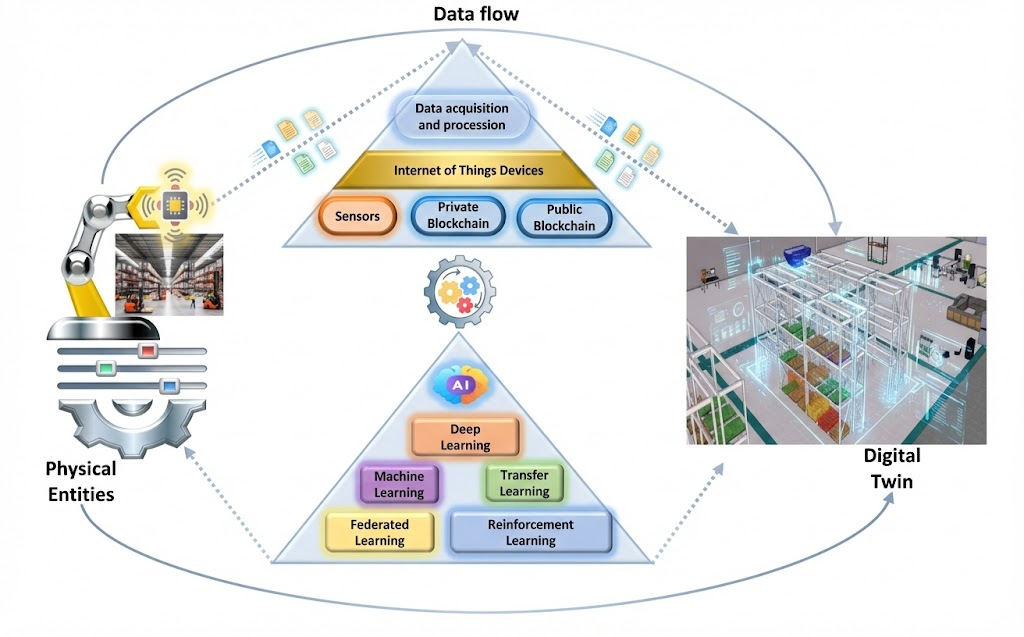
\includegraphics[width=0.98\textwidth]{images/system_intro.jpg}
\caption{\textcolor{blue}{Conceptual relationship between physical entities and the digital
twin, illustrating IoT-driven data acquisition, edge-level processing, and hybrid
blockchain integration for secure, verifiable lifecycle synchronization. The figure is enlarged across both columns to preserve labels and flow directions at print scale.}}
\label{fig:dt_concept}
\end{figure*}
Advancements in artificial intelligence (AI), machine learning (ML), and IoT technologies
have further expanded the capabilities of DT systems. AI- and ML-enhanced DTs have been
applied to optimize energy performance, improve predictive analytics, and strengthen
building operations, while IoT networks continuously deliver real-time contextual
data~\cite{sadri2023integration, zhang2025blockchain}. Despite these individual advancements, the
integration of these technologies with blockchain-based trust and provenance mechanisms
remains limited.
Research continues to report persistent challenges in cybersecurity, privacy protection,
and multi-layered information governance, indicating that current DT-integrated
architectures do not sufficiently support secure data handling, auditable governance, or
cross-domain verification~\cite{zhang2025blockchain, waheed2020security}.

\begin{table*}[!htbp]
\centering
\caption {Technical comparison between OrBIT and related works}
\label{tab:compare}
\scalebox{0.78}{
\begin{tabular}{p{1.3cm}p{4cm}p{3.2cm}p{3.2cm}p{3.5cm}p{3.2cm}}
\\ \hline\toprule
\textbf{Work}             & \textbf{Focus / Scope}                                                                & \textbf{Lifecycle Modeling}                                         & \textbf{Blockchain Architecture}                                     & \textbf{Intelligence \& Risk Handling}                                        & \textbf{Verification / Provenance}                                         \\ \hline\toprule
~\cite{suleiman2025blockchain}    & Security taxonomy for DT ecosystems                                                   & Partial (layer vulnerabilities only)                                & Generic blockchain layer                                             & None                                                                          & Immutability + event logging                                               \\ \hline
\cite{cunat2024blockchain}       & Blockchain enabled logistics DTs                                                      & None                                                                & Ethereum (public/permissioned)                                       & None                                                                          & Per entity provenance                                                      \\ \hline
\cite{suhail2024triple}          & TI supported DT security (TRIPLE)                                                     & None                                                                & Permissioned blockchain                                              & Partial (TI feed)                                                             & Rule based provenance                                                      \\ \hline
\cite{dai2024blockchain}         & Cryptographic DT access control                                                       & None                                                                & Hyperledger Fabric + IPFS                                            & None                                                                          & Strong (ABE based access proofs)                                           \\ \hline
\cite{samaniego2023digital}      & DT as proxy IoT privacy architecture                                                  & None                                                                & Ethereum private chain                                               & None                                                                          & Twin level hash verification                                               \\ \hline
\cite{du2025blockchain}          & Blockchain + DT state prediction for caching                                          & None                                                                & Permissioned blockchain + reputation                                 & DRL based optimization (domain specific)                                      & Signed caching records                                                     \\ \hline
\cite{swathi2025secure}          & Risk adaptive federated learning                                                      & None                                                                & Private blockchain (risk logs)                                       & Strong (risk adaptive FL + zk SNARKs)                                         & Model provenance + ZK verification                                         \\ \hline
\cite{akremi2025forensictwin}    & ForensicTwin evidence governance                                                      & Partial (forensic states)                                           & None                                                                 & None                                                                          & Forensic chain of custody + ontology checks                                \\ \hline
\textbf{OrBIT (Proposed)} & \textbf{Lifecycle-governed, blockchain-orchestrated DTs with deterministic
privacy routing} & \textbf{Full formal lifecycle with state transitions \& governance} & \textbf{Hybrid chain orchestration with multi layer trust anchoring} & \textbf{Deterministic policy-based privacy routing (HIPAA/GDPR/PCI)} & \textbf{Chain-anchored lifecycle verification + integrity-checked rollback} \\ \hline\toprule
\end{tabular}}
\end{table*}


These limitations impede adoption in safety-critical sectors, where deterministic provenance and real-time responsiveness are essential. Recent literature reviews and bibliometric analyses corroborate these observations, indicating that despite rapidly increasing interest in blockchain–digital twin (DT) integration, the field remains
conceptually fragmented. The absence of unified frameworks that incorporate lifecycle consistency and verifiable data
governance, as well as privacy-preserving data handling, combined with the lack of standardised definitions, synchronisation principles, and multi-domain architectural models, underscores the necessity for robust, orchestrated frameworks that facilitate transparent, accountable, and reliable DT ecosystems~\cite{ma2024examining}.
\smallskip
 
\noindent
\textcolor{blue}{Mission-critical DT ecosystems face three coupled security and reliability challenges:
(i)~data exposure across heterogeneous ledgers, which risks leaking confidential
operational parameters to public networks;
(ii)~non-deterministic or duplicate transaction commits, which undermine consistency in
multi-ledger environments; and
(iii)~the transaction cost of verifiable public anchoring, which limits scalability under
continuous telemetry flow. These concerns are operationally inseparable: a privacy decision controls the public effect, a crash can interrupt that effect after the private commit, and a slow public confirmation can delay clients unless coordination is explicitly asynchronous. We therefore ask whether deterministic routing prevents leakage, whether idempotent multi-relay delivery preserves exactly-once effects under crashes, and which ledger stage bounds latency in a geographically distributed deployment.
Existing DT blockchain frameworks improve traceability but fail to address these issues
holistically, often treating blockchain as a static storage backend rather than an
orchestrated execution layer.}
Motivated by these limitations, this work introduces OrBIT: an orchestrated digital twin
framework that integrates hybrid blockchain mechanisms with deterministic privacy routing
and verifiable lifecycle governance. OrBIT formalizes trusted data provenance, secures
lifecycle transitions, and enforces a deterministic, auditable privacy policy at the
DT--edge interface, thereby addressing the fragmentation, security weaknesses, and
transparency gaps identified across existing studies in Table~\ref{tab:compare}.
\textcolor{blue}{The key contributions of this paper are as follows:}
\begin{enumerate}
    \item \textcolor{blue}{We propose a unified hybrid-ledger architecture combining Hyperledger Fabric
    for private state management with Ethereum for public anchoring, treating blockchain
    provenance as an active control primitive. Anchoring is decoupled from ingestion by a
    transactional outbox, and exactly-once effects follow from composing an
    idempotency-keyed outbox, lease-coordinated relay workers, and an on-chain uniqueness check.}
    \item \textcolor{blue}{We design a deterministic, fail-closed privacy-routing policy grounded in
    established data-protection standards (HIPAA, GDPR, and PCI-DSS) that governs which
    fields may be written to the immutable public ledger. Because the decision is made by
    construction rather than by a probabilistic classifier, no field above the publication
    threshold can reach the public ledger, yielding a provable, auditable privacy
    guarantee rather than an estimated one.}
    \item \textcolor{blue}{We establish a mathematically defined lifecycle model with verifiable,
    append-only state transitions and integrity-checked rollback cryptographically bound
    to blockchain provenance, persisting history as reversible deltas with periodic
    checkpoints so that recovery cost is bounded by the checkpoint interval rather than by
    history depth.}
    \item \textcolor{blue}{We validate the architecture on four cloud VMs in two geographic regions under production WSGI serving, two-organization endorsement, controlled delay, block-cutting sweeps, synchronous and Fabric-only baselines, competing relay-coordination modes, four crash points, tampering, withholding, and reconciliation.}
\end{enumerate}
\textcolor{blue}{The measurements locate the dominant acknowledgement cost in Fabric ordering and quantify, rather than conceal, the remaining trust boundary: relay crashes are tolerated and externally auditable, whereas Byzantine ordering was not evaluated.}

The rest of the paper is organised as follows: Section~\ref{sec:review} explores previous approaches and provides insights about existing gaps addressed. Section~\ref{sec:system_design} presents the system architecture and methodology; Section~\ref{sec:results} discusses experimental results and performance evaluation; and Section~\ref{sec:conclusion} concludes the study with future directions.

\section{\textbf{Related Works}}
\label{sec:review}
\textcolor{blue}{Research on blockchain-enabled digital twins has expanded rapidly across cyber-physical infrastructures, driven by the need for trustworthy synchronisation, secure data exchange, and resilient decision intelligence. Early studies enhance DT security through decentralised trust models, with blockchain supporting integrity, provenance, and auditability. Suleiman et al.~\cite{suleiman2025blockchain}, for example, map attack surfaces across physical, data, model, and application layers, highlighting man-in-the-middle attacks, data poisoning, and model tampering. Cu\~nat et al.~\cite{cunat2024blockchain} show that Ethereum-based DLT integration can support verifiable IoT data flows but also identify performance and scalability limits when moving from permissioned storage to public anchoring. Table~\ref{tab:compare} compares representative state-of-the-art approaches.}

\textcolor{blue}{Beyond baseline security, DT research has progressed toward behaviour-aware protection. Suhail et al.~\cite{suhail2024triple} introduce TRIPLE, a DT-centric architecture combining blockchain provenance, threat intelligence, and hybrid modelling for continuous situational awareness. The approach remains primarily conceptual and does not define comprehensive lifecycle-governance semantics. Li et al.~\cite{li2023digital} identify interoperability, data trustworthiness, and architectural immaturity as barriers to robust blockchain-integrated DT deployment. Together, these studies motivate structured lifecycle management and multi-layer coordination.}

\textcolor{blue}{Recent surveys sharpen the security and deployment context of this problem. Laghari et al.~\cite{laghari2023blockchainiot} catalogue blockchain--IoT applications and identify interoperability, scalability, and multi-organisation security as persistent constraints; Jumani et al.~\cite{laghari2026blockchainsecurity} similarly organise blockchain threats, privacy mechanisms, and quality-of-service trade-offs. IoT reviews in gaming and multimedia environments~\cite{laghari2025gaming,laghari2025iomt} show that heterogeneous sensors generate latency-sensitive and privacy-sensitive streams beyond conventional industrial telemetry. These application domains motivate a routing and provenance layer whose safety properties do not depend on a learned classifier or a single workload distribution.}

\textcolor{blue}{The three additional works suggested during review occupy adjacent rather than directly competing layers. CardioTwin-XAI builds a federated predictive digital twin for cardiovascular care~\cite{yang2026cardiotwin}; FedLiverNet protects collaborative liver-image learning~\cite{lou2026fedlivernet}; and NeuroShield-Diabetes applies neural cryptography to health-data exchange~\cite{yang2026neuroshield}. They provide application- or model-level privacy mechanisms but do not specify a permissioned-to-public cross-chain commit protocol, relay coordination rule, or comparable end-to-end ledger workload. Treating their predictive accuracy or cryptographic cost as an OrBIT throughput baseline would therefore compare different dependent variables. We instead use three protocol-level baselines: Fabric-only ingestion, synchronous public anchoring, and uncoordinated race relays, with identical payloads and ledger topology.}

Access control and data governance are significant areas of focus in the DT security literature. Authors~\cite{dai2024blockchain} developed a CP ABE  and IPFS-enabled DT access control framework that provides fine-grained authorisation and efficient distributed storage. Although technically rigorous, this model prioritises cryptographic enforcement and does not address lifecycle-aware behavioural verification. Authors~\cite{samaniego2023digital}, through their digital twin as proxy architecture, positioned twins as intermediaries to prevent direct sensor access and maintain auditability using Ethereum-backed trust registries. While this model enhances IoT device privacy, it remains domain-restrictive and lacks orchestration logic for multi-twin governance. These studies reinforce the necessity for secure access governance that integrates DT semantics, evolving states, and operational context.

Other technically advanced contributions explore blockchain-driven optimisation and cyber resilience mechanisms within DT-enabled networks. Authors~\cite{du2025blockchain} designed a blockchain-empowered caching system enhanced with digital twin state prediction and reinforcement learning (PPO) to improve reliability and resource efficiency in D2D networks. Their approach demonstrates the potential of combining DT prediction with decentralised trust but remains confined to communication-level optimisation. Similarly, authors~\cite{swathi2025secure} introduced a federated, blockchain-secured, risk-adaptive deep learning framework to improve edge intelligence robustness, integrating zk SNARK verification, adversarial simulation, and energy-aware synchronisation. Although highly technical, it remains focused on federated learning rather than DT lifecycle coherence. These studies expose a growing interest in unifying intelligence, decentralisation, and behavioural modelling, yet none address the holistic governance challenges of multi-actor DT ecosystems.

Further research addresses forensics and global trends in DT–blockchain systems. Akremi’s ForensicTwin architecture incorporates forensic readiness attributes, such as provenance, integrity checks, and ontology-based evidence reasoning, directly into DT pipelines to ensure post-incident admissibility~\cite{akremi2025forensictwin}. Bibliometric studies, including those by authors~\cite{ma2024examining}, trace the evolution of DT blockchain research and identify persistent gaps in lifecycle governance, interoperability, and cross-domain orchestration. Authors~\cite{wakili2025digital} extend DT security into healthcare by combining Hyperledger-backed auditability with machine learning-driven anomaly detection, while author~\cite{louis2025advanced} synthesises DT IoT blockchain synergies within supply chain analytics, emphasising resilience and traceability. Authors~\cite{wang2023survey} present a comprehensive IoDT security taxonomy, introducing semantic communication threats, multi-twin attack surfaces, and vulnerabilities in decentralised intelligence. Collectively, these surveys demonstrate that technical advancements continue to outpace unified governance, lifecycle semantics, and cross-twin synchronisation standards.

\textcolor{blue}{Despite significant progress in these domains, current research lacks a lifecycle-governed,
blockchain-orchestrated digital twin architecture that delivers formalized state-transition
verification, hybrid-chain trust anchoring, and deterministic, auditable privacy governance
throughout the entire DT lifecycle. The proposed OrBIT framework addresses these gaps by
offering:}
\begin{enumerate}
    \item \textcolor{blue}{Formal DT lifecycle semantics with verifiable, append-only state transitions.}
    \item \textcolor{blue}{Hybrid-chain orchestration for verifiable trust anchoring with exactly-once cross-ledger effects under crash faults.}
    \item \textcolor{blue}{Deterministic, fail-closed privacy routing grounded in established data-protection standards, providing a by-construction guarantee on public-ledger exposure.}
    \item \textcolor{blue}{A distributed, multi-region evaluation that separates ingestion latency, public-ledger currency, and fault recovery.}
\end{enumerate}
\textcolor{blue}{OrBIT does not claim to replace a decentralised oracle or trustless bridge. Its relay workers are permissioned operational agents: leases prevent redundant submissions, while the Fabric record, Ethereum identifier uniqueness, and an independent auditor make omission or alteration detectable. A decentralised oracle network could consume the same outbox and commitment protocol, but would introduce a different validator and incentive model that is outside the present evaluation.}


% =====================================================================
% OrBIT — Section III, System Design & Methodology
% Rewritten to match the shipped implementation and the 19 Aug 2026 run
%   commit d8ce50b9 · config_hash bb85df0d7803 · server_mode production
%
% REMOVED FROM THIS SECTION — do not reinstate:
%   · \label{fig:flexsim_lab} and its figure (workspace merged.png)
%   · \label{tab:flexsim} (Table III, FlexSim parameters)
%   · subsection "FlexSim Digital Twin Simulation Dataset"
%   · the figure* block carrying \label{fig:c1_panel} — that figure now
%     lives in Section IV, and leaving it here duplicates the label
% =====================================================================

\section{\textbf{System Design \& Methodology}}
\label{sec:system_design}

\subsection{\textbf{System Architecture Overview}}
The proposed OrBIT architecture, illustrated in Figure~\ref{fig:system}, integrates five coordinated components into a deterministic and auditable pipeline. At the edge, a deterministic privacy policy engine evaluates each incoming digital twin payload at the field level and selects the appropriate processing path. Full payloads are handled by a permissioned Hyperledger Fabric network using channel isolation and multi-version concurrency control for secure and consistent storage. A public accountability layer on Ethereum records Keccak-based commitments through Merkle-batched anchors, ensuring tamper-evident verification without exposing sensitive content. An event-driven orchestrator assigns content-addressed identifiers, performs policy-driven routing, and enforces exactly-once effects across the two heterogeneous ledgers through a transactional outbox and an asynchronous relay worker. Finally, a digital twin manager maintains append-only versions via reversible deltas, periodic checkpoints, integrity-verified rollback, and DAG-based provenance for parent-to-child twin relationships. Together, these components deliver verifiable state transitions, provable privacy-preserving routing, and end-to-end integrity across the digital twin lifecycle.

\begin{figure*}[!htbp]
\centering
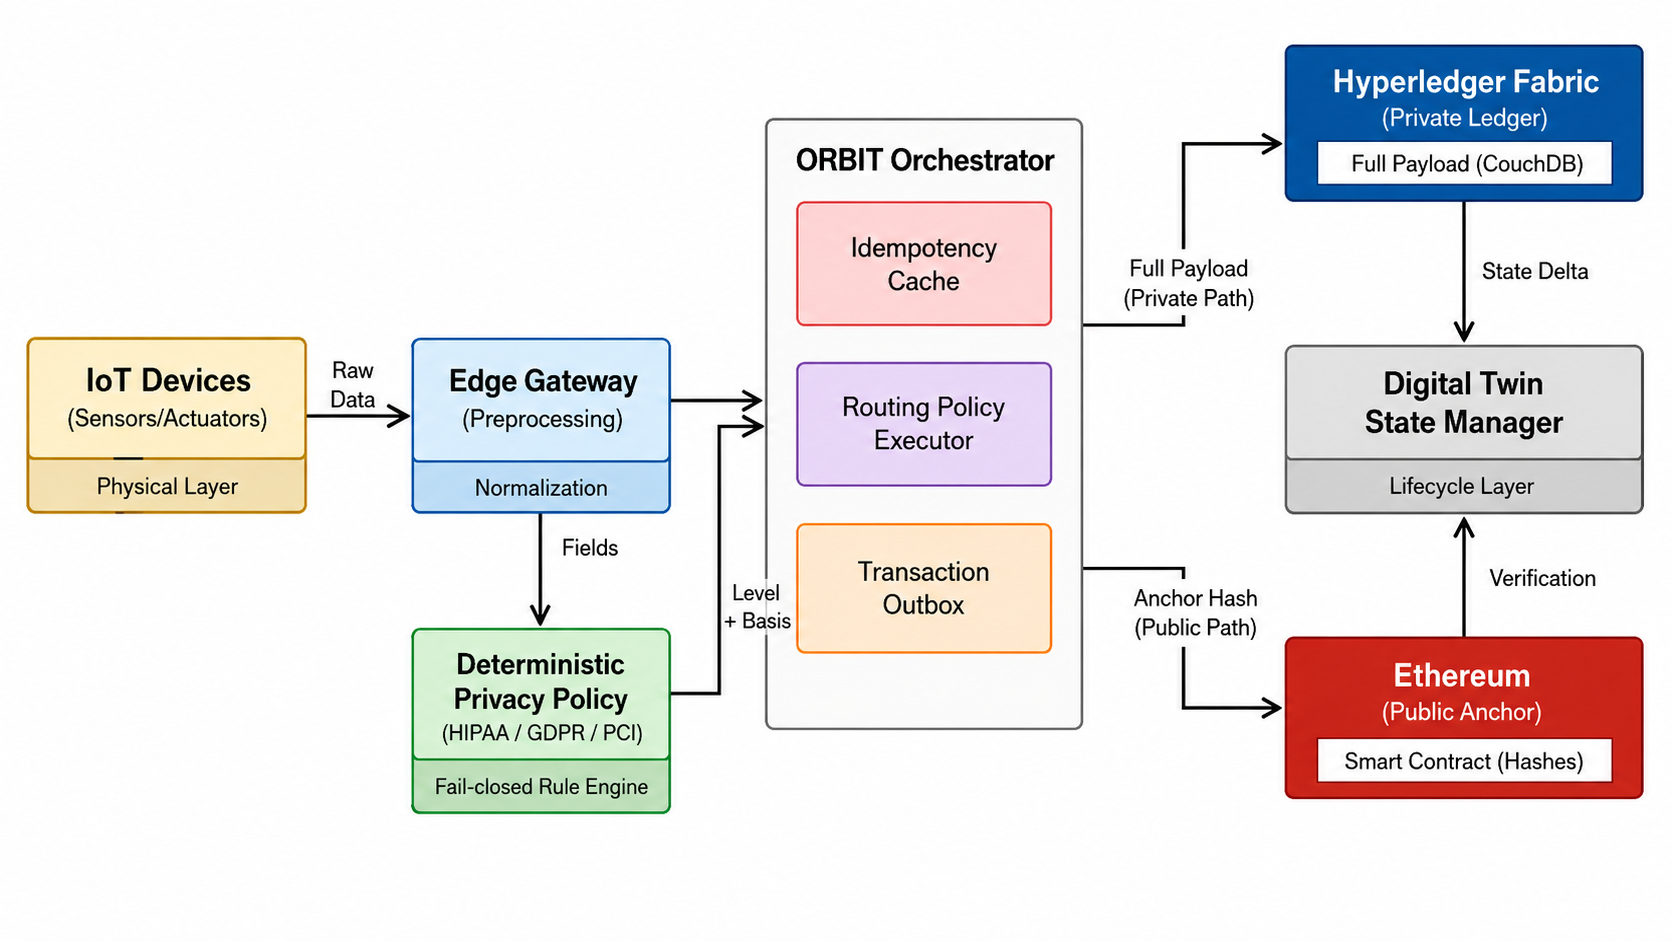
\includegraphics[width=0.8\textwidth]{images/system_arch.png}
\caption{Functional architecture of the OrBIT framework. The pipeline processes IoT
telemetry through three stages: (1)~a deterministic privacy policy engine that assigns each
field a sensitivity level from name- and value-based rules grounded in
HIPAA/GDPR/PCI-DSS, failing closed for unrecognized fields; (2)~orchestration, where an
idempotency-aware executor performs policy-driven routing and enforces exactly-once
effects; and (3)~hybrid storage, where the full payload is committed to Hyperledger Fabric
(private path) while redacted commitments are Merkle-batched and anchored on Ethereum
(public path).}
\label{fig:system}
\end{figure*}

\subsection{\textbf{Deterministic Privacy Policy Engine}}
\label{sec:policy}

Routing decisions in OrBIT determine whether a data field may be written to an immutable public ledger. Because such a write is irreversible, this decision is made by a deterministic, auditable policy rather than a probabilistic classifier: a single misclassification would permanently anchor sensitive data in public, and no confidence threshold can bound that risk after the fact. OrBIT therefore replaces statistical inference on the privacy-critical path with an explicit field-sensitivity policy whose behaviour is fixed, reproducible, and independently verifiable.

Each incoming payload $\mathbf{x}$ is modelled as a set of named fields $\{(k_1,v_1),\ldots,(k_n,v_n)\}$, where $k_j$ is a field name and $v_j$ its value. The policy engine assigns to every field an ordered sensitivity level
\begin{equation}
\scriptsize
  \ell(k_j,v_j)\in\mathcal{L}=\{\textsc{public}\prec\textsc{restricted}\prec\textsc{confidential}\prec\textsc{critical}\},
  \label{eq:levels}
\end{equation}
by evaluating two rule families in sequence. First, a name-based rule set $\mathcal{R}_{\mathrm{name}}$ maps field names to sensitivity levels using a declared table grounded in established data-protection standards, namely HIPAA identifiers, GDPR Article~9 special categories, and PCI-DSS cardholder data. Second, a value-based rule set $\mathcal{R}_{\mathrm{val}}$ inspects field values against pattern matchers (e.g., national identifiers, e-mail addresses, and payment-card numbers) and escalates the assigned level when a sensitive pattern is detected. The engine takes the more restrictive of the two outcomes,
\begin{equation}
\scriptsize
  \ell(k_j,v_j)
  = \max\!\big(\,\ell_{\mathrm{name}}(k_j),\ \ell_{\mathrm{val}}(v_j)\,\big),
  \label{eq:escalation}
\end{equation}
where $\max$ is taken over the total order in~\eqref{eq:levels}. Any field that matches no rule receives the most restrictive level by default,
\begin{equation}
\scriptsize
  \ell(k_j,v_j)=\textsc{critical}
  \quad\text{if}\quad
  k_j\notin\mathrm{dom}(\mathcal{R}_{\mathrm{name}})
  \ \wedge\
  v_j\notin\mathrm{dom}(\mathcal{R}_{\mathrm{val}}),
  \label{eq:failclosed}
\end{equation}
so the policy is \emph{total} (defined for every field) and \emph{fail-closed} (an unrecognized field is never published). This property directly bounds the public-exposure surface: a field can reach the public ledger only if an explicit rule declares it publishable.

The declared rule table includes device and schema identifiers at the \textsc{public} level, since an anchor that carries no identifying metadata cannot be reconciled against off-chain records by an auditor. This is a deliberate policy choice with a visible consequence---device-level activity becomes externally observable---and where device identifiers are themselves quasi-identifying, the rule table is the correct place to reclassify them. The fail-closed default guarantees that any field not explicitly declared publishable is withheld regardless.

\paragraph*{\textbf{Ledger routing.}}
Let $\theta=\textsc{public}$ denote the publication threshold. The routing function partitions each payload into the private component committed to the permissioned ledger and the public component eligible for anchoring:
\begin{equation}
\scriptsize
  R(\mathbf{x})
  =
  \Big\langle
    \underbrace{\mathbf{x}}_{\text{Fabric (private)}},\;
    \underbrace{P=\{(k_j,v_j): \ell(k_j,v_j)=\theta\}}_{\text{Ethereum (public)}}
  \Big\rangle.
  \label{eq:routing}
\end{equation}
The full payload is \emph{always} committed to the permissioned ledger, without regard to sensitivity, so no field is lost at rest; only fields at the \textsc{public} level contribute to the redacted metadata anchored publicly. Consequently, no field whose level exceeds $\theta$ can appear in the public commitment, which establishes the privacy guarantee by construction rather than by empirical estimation. When $P=\varnothing$ the record has no publishable content and no anchor is produced; this is the \texttt{FABRIC\_ONLY} branch of Algorithm~\ref{alg:routing}, and Section~\ref{sec:res_orch} reports it as a measured routing path rather than a design possibility.

\paragraph*{\textbf{Auditability.}}
Every field decision is emitted with the identifier of the rule that produced it and the standard on which that rule is based, yielding a per-record decision log
\begin{equation}
  \mathcal{A}(\mathbf{x})
  = \big\{\,\langle k_j,\ \ell(k_j,v_j),\ \mathrm{rule\_id}_j,\ \mathrm{basis}_j\rangle\,\big\}_{j=1}^{n},
  \label{eq:audit}
\end{equation}
which records both the level assigned to each field and, for withheld fields, the reason for redaction. Because the policy is deterministic, the same payload always yields the same decision log, so routing behaviour is fully reproducible and can be re-verified offline against~\eqref{eq:escalation}--\eqref{eq:routing}. The ordered scale in~\eqref{eq:levels} is additionally reused by a role-based access matrix that governs how much of a stored private record is disclosed in response to an authorized query, as described in Section~\ref{sec:fabric}.

\subsection{\textbf{Hyperledger Fabric Private Blockchain Layer}}
\label{sec:fabric}

The permissioned ledger is implemented on Hyperledger Fabric, modelled here as a key--versioned state machine replicated across peers and advanced through an endorse--order--validate--commit pipeline. Let $\mathcal{K}$ denote the application key space, and let the world state at block height $h$ be the mapping $S_h:\mathcal{K}\to\mathbb{V}\times\mathbb{N}$, with each key $k$ storing a value--version pair $(v,\nu)$. A chaincode invocation $tx$ produces a read set $R=\{(k,\nu_k)\}$ and a write set $W=\{(k,v_k^\star)\}$. Transaction validity at height $h{+}1$ requires (i) satisfaction of the endorsement policy and (ii) multi-version concurrency control (MVCC):
\begin{subequations}
\begin{align}
&\forall\,e\in\mathcal{E}^\star:\
   \mathrm{VerifySig}_e(\mathrm{digest}(tx))=1, \label{eq:fabric_endorse}\\
&\forall\,(k,\nu_k)\in R:\
   S_h(k)=(\cdot,\nu_k), \label{eq:fabric_mvcc}
\end{align}
\end{subequations}
where $\mathcal{E}^\star$ is the set of endorsers specified by policy $\mathsf{P}$ (e.g., $\mathsf{AND}(\mathrm{Org}_1,\mathrm{Org}_2)$ or $t$-of-$n$). Endorsements are X.509/MSP-anchored signatures over proposal digests, providing Byzantine tamper evidence under Fabric's identity model.

\paragraph*{\textbf{Ordering and block cutting.}}
Ordering is provided by Raft, treated as a leader-based crash-fault-tolerant (CFT) consensus protocol. The commit latency is well approximated by
\begin{equation}
T_{\mathrm{commit}}
\approx
T_{\mathrm{endorse}}
+ T_{\mathrm{order}}
+ T_{\mathrm{validate}}
+ T_{\mathrm{apply}},
\label{eq:commit_lat}
\end{equation}
where the components correspond respectively to proposal dissemination, block replication, policy and MVCC checks, and state-database writes.

The ordering service cuts a block on whichever of two conditions is met first: the batch timeout $\Delta_{\mathrm{to}}$ elapses, or the number of pending transactions reaches the maximum message count $B_{\max}$. Under a closed-loop client population of size $c$, the orderer observes $c$ pending messages, so the governing condition is
\begin{equation}
  \text{block cut on count} \iff c \ge B_{\max},
  \label{eq:block_cut}
\end{equation}
and the acknowledgement latency floor below that threshold is $\Delta_{\mathrm{to}}$ plus endorsement, validation and commit. This gives two distinct operating regimes---timeout-dominated below $B_{\max}$ and arrival-rate-dominated above it---and the transition is a configuration boundary rather than a property of the architecture. Sustainable throughput accordingly satisfies
\begin{equation}
\mathrm{TPS}_{\mathrm{fabric}}
 \le
 \min\!\Big\{\frac{B}{\Delta_b},\
                 \frac{1}{\mathbb{E}[T_{\mathrm{validate}}+T_{\mathrm{apply}}]}\Big\},
\label{eq:tps_fabric}
\end{equation}
for average block size $B$ and inter-block interval $\Delta_b$. Section~\ref{sec:res_orch} measures both regimes and locates the transition against the channel configuration reported in Section~\ref{sec:ledger_config}.

Because Fabric uses optimistic concurrency, write conflicts occur when two transactions read the same key and at least one updates it before commit. If accesses to a hot key $k$ follow a Poisson process with rate $\lambda_k$ and the average validation window is $\Delta_v$, a first-order contention estimate is
\begin{subequations}
\begin{align}
\Pr[\mathrm{abort\ on}\ k] &\approx 1 - e^{-\lambda_k\Delta_v}, \label{eq:abort}\\
\Pr[\mathrm{commit}]
   &\approx \prod_{(k,\cdot)\in R} e^{-\lambda_k\Delta_v}.
   \label{eq:commit_prob}
\end{align}
\end{subequations}
These relations motivate two engineering strategies adopted in our chaincode design: (i) \emph{key sharding}, which decomposes composite resources into finer-grained keys to reduce contention rates $\lambda_k$; and (ii) \emph{idempotent upserts} with read-less writes for append-only records, minimizing $|R|$ and improving~\eqref{eq:commit_prob}. We note that~\eqref{eq:abort}--\eqref{eq:commit_prob} are design-guiding estimates; the single-writer workload evaluated here does not exercise key contention, and we make no measured claim about them.

Privacy at the storage layer is enforced through channel isolation and role-based disclosure. The chaincode persists the complete payload on the permissioned ledger, so no field is lost at rest, while the public world state receives only the cryptographic commitment of a record rather than its plaintext:
\begin{subequations}
\begin{align}
\text{Public commitment:} \quad
  &S_{h+1}(k)=\big(\mathrm{hash}(m),\,\nu{+}1\big), \label{eq:public_hash} \\
\text{Private record:} \quad
  &k \mapsto m. \label{eq:private_record}
\end{align}
\end{subequations}
This hash-anchor pattern ensures auditability and referential integrity without revealing plaintext. When an authorized party queries a stored record, disclosure is governed by a role-based access matrix over the sensitivity scale of~\eqref{eq:levels}: a requester is served only those fields whose level is permitted for its role, and all other fields are redacted. This query-time gate is reversible and therefore distinct from the irreversible publication gate of Section~\ref{sec:policy}; it is implemented alongside the publication policy but is not exercised by the experiments reported here. Access control lists (ACLs) tied to chaincode namespaces enforce that an identity may invoke a privileged operation only if
\begin{equation}
\mathsf{Q}(\mathrm{id})=1 \ \land\ \mathsf{P}(tx)=1,
\label{eq:auth_cond}
\end{equation}
yielding a compositional authorization condition. Together, these mechanisms provide consistent, access-controlled storage for restricted, confidential, and critical payloads, while supplying cryptographically verifiable state transitions suitable for external anchoring and cross-system reconciliation.

\subsection{\textbf{Ethereum Public Blockchain Layer}}
\label{sec:eth}

The public layer provides transparency and non-repudiation by anchoring redacted, non-sensitive metadata as cryptographic commitments on Ethereum. Let $m$ denote a deterministic metadata digest (e.g., schema identifier, device identifier, timestamp, and integrity tag) derived from the publishable fields of the payload $\mathbf{x}$. A collision-resistant commitment is computed via Keccak-256,
\begin{equation}
  h = \mathcal{H}(m),
  \label{eq:eth_hash}
\end{equation}
and stored on-chain as part of a registry tuple $(\texttt{id},h,\tau,\texttt{owner})$. Because the underlying content is never revealed, an auditor verifies integrity by recomputing $h'$ from independently obtained metadata $m_{\text{off}}$ and checking the equality $h'=h$.

To reduce per-record gas cost, batches $\{m_i\}_{i=1}^{N}$ are aggregated into a Merkle tree whose root is the sole on-chain commitment:
\begin{subequations}
\begin{gather}
R = \mathrm{MerkleRoot}\!\big(\{\mathcal{H}(m_i)\}_{i=1}^{N}\big), \label{eq:root}\\
\mathrm{VerifyMerkle}\!\big(R,\mathcal{H}(m_j),\pi_j\big)=\textsf{true}, \label{eq:verify}
\end{gather}
\end{subequations}
where $\pi_j$ is a standard Merkle proof of length $\lceil \log_2 N\rceil$. This provides a publicly verifiable audit trail without leaking the private content stored in the permissioned ledger. The proof is the verification cost transferred to the auditor in exchange for the operator's gas saving, and Section~\ref{sec:res_gas} reports both sides of that exchange.

The contract maintains a minimal mapping $\mathcal{M}:\texttt{bytes32}\!\rightarrow\!\textsf{Record}$, where each \textsf{Record} contains $(h,\tau,\texttt{owner})$. A transaction $tx$ invoking \texttt{registerData(id,}$h$\texttt{,\ldots)} is valid only if (i) $\mathcal{M}(\texttt{id})$ is empty and (ii) the caller satisfies an authorization predicate $\mathsf{Auth}(\cdot)=1$ (owner/role gating). Condition~(i) is enforced on chain by an explicit uniqueness check that reverts on a repeated identifier,
\begin{equation}
  \mathcal{M}(\texttt{id}) = \varnothing
  \quad\text{(else revert)},
  \label{eq:onchain_unique}
\end{equation}
and is not merely a convention of the calling client. As Section~\ref{sec:orchestrator} shows, \eqref{eq:onchain_unique} is one of the two mechanisms that together yield exactly-once effects across the ledgers.

The approximate gas cost for a single-item commit is
\begin{equation}
\scriptsize
G_{\text{tx}} \approx G_0
  + n_{\text{SSTORE}}\,G_{\text{SSTORE}}
  + n_{\text{LOG}}\,G_{\text{LOG}}
  + \alpha\,|m|,
\label{eq:gas_single}
\end{equation}
where $G_0$ is the intrinsic base cost, $G_{\text{SSTORE}}$ accounts for persistent writes, $G_{\text{LOG}}$ covers event emission, and the linear term reflects calldata size. For batched commits, only the root is written on chain, so the numerator is independent of $N$ and the amortized gas per item satisfies
\begin{equation}
\bar{G}_{\text{item}}(N)
\approx
\frac{G_{\text{root}}}{N},
\qquad
\frac{\partial G_{\text{root}}}{\partial N}\approx 0.
\label{eq:gas_batch}
\end{equation}
The independence of $G_{\text{root}}$ from $N$ is the property on which the entire batching argument rests, and it is measured rather than assumed in Section~\ref{sec:res_gas}. Given block gas limit $L_g$, mean per-transaction gas $\bar{g}$, and average block interval $\Delta_b$, registry throughput is bounded by
\begin{equation}
\mathrm{TPS}_{\text{eth}}
\le
\frac{L_g}{\bar{g}\,\Delta_b}.
\label{eq:eth_tps}
\end{equation}

To quantify the efficiency gained through Merkle batching, we define the gas-reduction ratio relative to the single-item anchoring baseline. Let $G_{\text{single}}$ denote the gas cost of anchoring one record individually (Eq.~\ref{eq:gas_single}), and let $\bar{G}_{\text{item}}(N)$ denote the amortized gas cost per record when batching $N$ items (Eq.~\ref{eq:gas_batch}). The reduction achieved at batch size $N$ is
\begin{equation}
\mathrm{Reduction}(N)
=
1 - \frac{\bar{G}_{\text{item}}(N)}{G_{\text{single}}}.
\label{eq:gas_reduction}
\end{equation}
Because the batching path and the single-record path have different fixed costs, \eqref{eq:gas_reduction} is not positive for all $N$: there exists a crossover
\begin{equation}
  N^\star = \Big\lceil \frac{G_{\text{root}}}{G_{\text{single}}} \Big\rceil,
  \label{eq:gas_crossover}
\end{equation}
below which batching is a net cost. Above $N^\star$ the reduction rises as $1-G_{\text{root}}/(N\,G_{\text{single}})$ with diminishing marginal returns, while the proof length grows as $\lceil\log_2 N\rceil$; together with anchoring-latency constraints this yields an optimal operating region rather than unbounded batching. Section~\ref{sec:res_gas} reports $N^\star$ as measured.

Finality depends on the confirmation depth $z$, giving expected confirmation time
\begin{equation}
T_{\text{final}} \approx z\,\Delta_b,
\label{eq:finality}
\end{equation}
and producing a cross-chain visibility interval of
\begin{equation}
T_{\text{cross}}
=
T_{\text{fabric commit}}
+ T_{\text{queue}}
+ T_{\text{relay}}
+ T_{\text{final}},
\label{eq:cross_sla}
\end{equation}
where $T_{\text{queue}}$ is the interval an outbox event waits before the relay worker collects it. Separating $T_{\text{queue}}$ from $T_{\text{relay}}$ matters because the two respond differently to load: the chain call is roughly constant while the queue term grows once the offered rate exceeds the relay's drain rate.

To bind the permissioned and public layers, each Fabric commit of key $k$ with version $\nu$ and timestamp $\tau$ emits a relay tuple
\[
\sigma = \langle k,\nu,\tau,\mathcal{H}(m)\rangle,
\]
whose digest is anchored on Ethereum:
\begin{subequations}
\scriptsize
\begin{align}
c &= \mathcal{H}(\sigma), \label{eq:anchor_c}\\
c' &= \mathcal{H}\!\left(\langle k,\nu,\tau,\mathcal{H}(m)\rangle\right),\quad c'=c \ \text{(audit check)}. \label{eq:anchor_eq}
\end{align}
\end{subequations}
Equality of $c$ and $c'$ ensures end-to-end non-repudiation: any alteration in either ledger breaks the commitment.

Security on Ethereum is maintained through immutability, replay protection (nonce and chain-id binding), and a minimal stateful interface. The contract adheres to checks--effects--interactions ordering and avoids external calls in state-modifying functions to eliminate reentrancy risk. Identifiers are normalized to fixed-width \texttt{bytes32} to prevent unintended storage growth, and metadata is emitted primarily via events for gas efficiency. Combined, the commitment rule~\eqref{eq:eth_hash}, the uniqueness check~\eqref{eq:onchain_unique}, the gas-aware design~\eqref{eq:gas_single}--\eqref{eq:eth_tps}, and the cross-chain anchoring logic~\eqref{eq:anchor_c}--\eqref{eq:anchor_eq} yield an auditable, cost-efficient public accountability layer that complements the permissioned ledger without exposing private payloads.

\subsection{\textbf{Orchestrator Integration Layer}}
\label{sec:orchestrator}

The OrBIT orchestrator is an event-driven microservice that implements the end-to-end control plane for secure ingestion, policy evaluation, routing, and hybrid-ledger coordination, as illustrated in Figure~\ref{fig:orbit_sequence}. The sequence makes the consistency boundary explicit: the client is acknowledged after the private commit and durable outbox insertion, whereas public anchoring proceeds independently. Each telemetry payload $\mathbf{x}$ is submitted by an IoT device via a REST interface and timestamped at ingress time $t_0$. Upon reception, the orchestrator deterministically derives a content-addressed identifier
\begin{equation}
  \texttt{id}=\mathcal{H}(\mathbf{x}\Vert t_0),
  \label{eq:orc_id}
\end{equation}
which serves as a global idempotency key and uniquely identifies the request across retries, crashes, and cross-chain effects (Fig.~\ref{fig:orbit_sequence}, Steps~1--1b).

\begin{figure*}[!htbp]
\centering
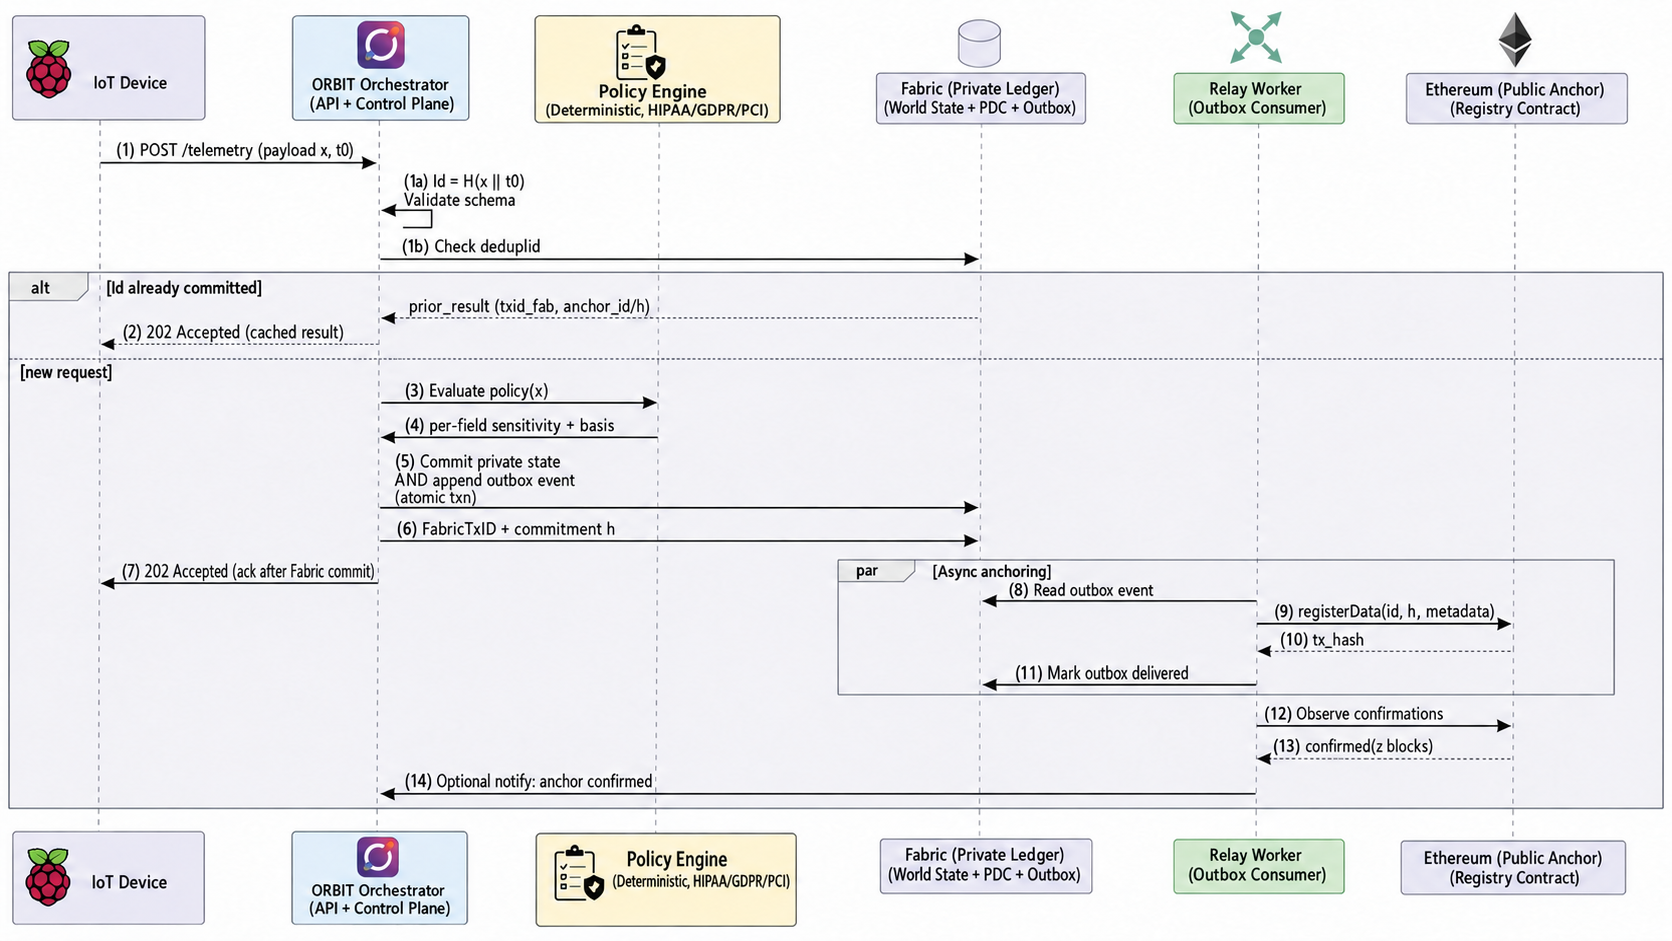
\includegraphics[width=0.90\textwidth]{images/orchestra_v2.png}
\caption{Detailed orchestration sequence and consistency protocol. Exactly-once delivery is ensured by an idempotency check (Steps 1a--2) before processing. Latency is bounded by acknowledging the client with \texttt{202 Accepted} (Step 7) immediately after the private Fabric commit (Step 5), decoupling the slower public anchoring (Steps 8--13) into an asynchronous background process via the transactional-outbox pattern. Routing is determined by the deterministic policy engine (Steps 3--4), which returns each field's sensitivity level and legal basis rather than a probabilistic classification.}
\label{fig:orbit_sequence}
\end{figure*}

\paragraph*{\textbf{Idempotent ingress and fast-path acknowledgement}}
Before any side effects are executed, the orchestrator checks whether \texttt{id} already exists in a persistent deduplication set $\mathcal{D}$. If the identifier is found, the orchestrator immediately returns a cached response containing the previously issued Fabric transaction identifier and anchor commitment, without re-evaluating the policy or repeating ledger writes (Fig.~\ref{fig:orbit_sequence}, \textit{alt} path). This mechanism enforces exactly-once semantics under retries while providing fast responses for duplicate submissions.

\paragraph*{\textbf{Policy-driven routing and private commit}}
For a new request ($\texttt{id}\notin\mathcal{D}$), the payload is evaluated by the deterministic privacy policy engine of Section~\ref{sec:policy}, which returns the per-field sensitivity assignment and the resulting publishable set $P$ (Fig.~\ref{fig:orbit_sequence}, Steps~3--4). The orchestrator then commits the full payload to the permissioned ledger through a real chaincode invocation. The Fabric write is issued via the operator-standard \texttt{peer} command-line interface against channel \texttt{hiot}, invoking the \texttt{StoreIoTData} chaincode and reading the record back to confirm persistence; the real transaction identifier returned by the ledger is retained for the client response and the audit trail. A failed private commit is fatal to the request: the orchestrator releases the idempotency slot and returns an error rather than anchoring a commitment for a record that does not exist at rest.

If $P\neq\varnothing$, an outbox event $\sigma$ is appended to a durable append-only log,
\begin{equation}
  \sigma=\langle \texttt{id}, k, \nu, \tau, \mathcal{H}(m)\rangle,
  \label{eq:sigma}
\end{equation}
so that the private state mutation and the intent to publish accountability metadata are recorded together (Fig.~\ref{fig:orbit_sequence}, Step~5). The outbox row and the deduplication record are written in a single local transaction, and the outbox is keyed on \texttt{id}, so a duplicate submission cannot enqueue a second anchor.

Upon successful validation and commit, the orchestrator returns a \texttt{202~Accepted} acknowledgement to the client containing the Fabric transaction identifier, the commitment hash, and an outbox handle by which anchor progress may be polled (Step~7). This acknowledgement is issued \emph{before} public anchoring begins, bounding ingestion latency independently of Ethereum confirmation delays; the response therefore does not and cannot carry an Ethereum transaction hash.

\paragraph*{\textbf{Asynchronous anchoring and exactly-once effects}}
\textcolor{blue}{Public anchoring is decoupled from the ingestion path via the transactional outbox. One or more independently restartable relay processes poll pending events. In the coordinated mode evaluated here, a relay atomically acquires a time-bounded lease before submitting an event; an expired lease makes abandoned work eligible for another process. The winning relay registers the commitment on Ethereum and records the receipt (Fig.~\ref{fig:orbit_sequence}, Steps~8--11), while transient failures are retried with exponential backoff. Confirmation monitoring proceeds independently until a depth of $z$ blocks is observed, after which optional client notifications may be emitted (Steps~12--14). The lease prevents redundant transactions during normal operation but is not itself the safety boundary.}

\textcolor{blue}{Exactly-once \emph{effects} arise from three mechanisms acting together. The outbox key prevents duplicate enqueueing; relay leases allocate pending work without relying on one continuously available process; and the on-chain uniqueness check~\eqref{eq:onchain_unique} closes the crash window between transaction broadcast and receipt persistence. A restarted relay first queries the registry and treats an already-registered identifier as successful delivery. At-least-once delivery composed with on-chain uniqueness therefore yields an exactly-once effect,}
\begin{equation}
  \big|\{\text{anchors}(\texttt{id})\}\big| = 1
  \quad \forall\ \texttt{id} \ \text{with}\ P\neq\varnothing.
  \label{eq:exactly_once_effect}
\end{equation}

\paragraph*{\textbf{Consistency boundary}}
\textcolor{blue}{Hyperledger Fabric and the local outbox store cannot participate in a common transaction, so the private commit and outbox insertion are ordered rather than atomic: Fabric commit, then outbox row and deduplication record in one local transaction, then acknowledgement. A crash in the intervening window can leave a privately committed record without an outbox row. We do not claim cross-ledger atomicity. A reconciliation sweep enumerates Fabric records, compares them with the deduplication and outbox tables, recreates missing intents, and lets the ordinary lease protocol deliver them. A standalone auditor recomputes each commitment from Fabric state and compares the result with the Ethereum registry, thereby detecting both alteration and withholding independently of the relay process.}

\begin{algorithm}[!htbp]
\scriptsize
\caption{\textcolor{blue}{Pseudocode for lease-coordinated relay delivery and reconciliation}}
\label{alg:relay}
\KwData{\textcolor{blue}{Durable outbox $\mathcal{O}$; relay identifier $r$; lease duration $\ell$; Fabric records $\mathcal{F}$; Ethereum registry $\mathcal{M}$}}
\KwResult{\textcolor{blue}{One durable public effect for every publishable committed record}}
\While{\textcolor{blue}{relay $r$ is running}}{
  \textcolor{blue}{Atomically claim one pending or expired row $o\in\mathcal{O}$ until $t+\ell$}\;
  \If{\textcolor{blue}{no row is claimable}}{\textcolor{blue}{wait with backoff; continue}\;}
  \If{\textcolor{blue}{$\mathcal{M}$ already contains $o.\mathtt{id}$}}{
    \textcolor{blue}{mark $o$ delivered and persist the observed receipt}\;
  }
  \Else{
    \textcolor{blue}{submit $\langle o.\mathtt{id},o.\mathtt{commitment}\rangle$ to Ethereum}\;
    \textcolor{blue}{persist the receipt; mark $o$ delivered}\;
  }
}
\ForEach{\textcolor{blue}{$f\in\mathcal{F}$ during reconciliation}}{
  \If{\textcolor{blue}{$f$ is publishable and has no outbox intent}}{
    \textcolor{blue}{recompute and insert the missing intent idempotently}\;
  }
}
\textcolor{blue}{Audit by recomputing each Fabric commitment and comparing it with $\mathcal{M}$}\;
\end{algorithm}

\paragraph*{\textbf{Latency and throughput model}}
The client-visible pipeline is a composition of preprocessing (\textsf{prep}), policy evaluation (\textsf{pol}), private ledger commit (\textsf{fab}), and outbox insertion (\textsf{obx}). Public anchoring lies outside it. Two latencies are therefore distinguished:
\begin{subequations}
\small
\begin{align}
  T_{\mathrm{ack}}(\mathbf{x})
    &= T_{\mathrm{prep}}+T_{\mathrm{pol}}+T_{\mathrm{fab}}+T_{\mathrm{obx}},
    \label{eq:t_ack}\\
  T_{\mathrm{cmp}}(\mathbf{x})
    &= T_{\mathrm{ack}}+T_{\mathrm{queue}}+T_{\mathrm{eth}}^{\mathrm{anchor}},
    \label{eq:t_cmp}
\end{align}
\end{subequations}
where $T_{\mathrm{ack}}$ is the acknowledgement latency observed by the client and $T_{\mathrm{cmp}}$ is the completion latency until the anchor is durable on the public ledger. For a record with $P=\varnothing$, $T_{\mathrm{cmp}}=T_{\mathrm{ack}}$ and no anchor is produced. Reporting the two separately is necessary rather than cosmetic: quoting $T_{\mathrm{cmp}}$ as though it were the chain cost conflates queue wait with anchoring work.

Under steady-state arrival rate $\lambda$, throughput is bounded by the slowest stage:
\begin{subequations}
\small
\begin{align}
  \mathrm{TPS}_{\mathrm{orch}} &\le \min_s \mu_s, \label{eq:tps_orch}\\
  \rho_s &= \lambda/\mu_s < 1. \label{eq:util}
\end{align}
\end{subequations}
Two distinct ceilings follow. Ingestion throughput is bounded by the private-commit stage, itself governed by the block-cutting condition~\eqref{eq:block_cut}. Public-ledger currency is bounded independently by the relay's drain rate $\mu_{\mathrm{relay}}$, so that a backlog forms whenever $\lambda > \mu_{\mathrm{relay}}$ and $T_{\mathrm{queue}}$ grows accordingly. Both ceilings are measured in Section~\ref{sec:res_orch}.

\paragraph*{\textbf{Exactly-once correctness condition}}
Formally, a request is committed if and only if
\begin{equation}
\small
  \mathsf{Commit}(\mathbf{x},\texttt{id})
  =
  (\texttt{id}\notin\mathcal{D})
  \land \mathsf{Auth}(\mathrm{caller})
  \land \mathsf{Valid}(\mathbf{x}),
  \label{eq:commit}
\end{equation}
and all downstream effects (the Fabric state update, the outbox emission, and the Ethereum anchoring) are causally linked to this single decision. The combination of idempotent ingress, an idempotency-keyed outbox, and on-chain identifier uniqueness ensures that OrBIT enforces exactly-once effects across the private and public ledgers, as operationalized in Algorithm~\ref{alg:routing}.

\begin{algorithm}[!htbp]
\scriptsize
\caption{\textcolor{blue}{Pseudocode for deterministic policy-driven routing and commit}}
\label{alg:routing}
\KwData{$\mathtt{Incoming\ Payload:}$ $\mathbf{x}=\{(k_j,v_j)\}$; $\mathtt{Arrival\ Time:}$ $t_0$; $\mathtt{Name\ Rules:}$ $\mathcal{R}_{\mathrm{name}}$; $\mathtt{Value\ Rules:}$ $\mathcal{R}_{\mathrm{val}}$; $\mathtt{Publication\ Threshold:}$ $\theta$}
\KwResult{$\mathtt{Ledger\ Commit\ Confirmation}$; $\mathtt{Client\ Notification}$; $\mathtt{Routing\ Path}$}
Initialize deduplication store $\mathcal{D}$, outbox $\mathcal{O}$, ledger connections \\
\BlankLine
Begin: \\
\textbf{Idempotency Check:} \\
Compute idempotency key $\texttt{id} \leftarrow \mathcal{H}(\mathbf{x}\Vert t_0)$ \\
\If{$\texttt{id} \in \mathcal{D}$} {
    Retrieve cached result $\mathcal{R}_{\text{cached}} \leftarrow \mathcal{D}[\texttt{id}]$ \\
    \textbf{Return} $\langle\mathtt{DUPLICATE}, \mathcal{R}_{\text{cached}}\rangle$ \\
}
\BlankLine
\textbf{Deterministic Field Classification:} \\
Initialize decision log $\mathcal{A} \leftarrow \varnothing$, public set $P \leftarrow \varnothing$ \\
\For{$\mathtt{each\ field}$ $(k_j,v_j) \in \mathbf{x}$} {
    $\ell_{\mathrm{name}} \leftarrow \mathcal{R}_{\mathrm{name}}(k_j)$ \tcp*{$\textsc{critical}$ if unmatched}
    $\ell_{\mathrm{val}}  \leftarrow \mathcal{R}_{\mathrm{val}}(v_j)$ \tcp*{$\textsc{public}$ if unmatched}
    $\ell_j \leftarrow \max(\ell_{\mathrm{name}}, \ell_{\mathrm{val}})$ \tcp*{fail-closed to $\textsc{critical}$}
    Record $\langle k_j, \ell_j, \mathrm{rule\_id}_j, \mathrm{basis}_j\rangle$ in $\mathcal{A}$ \\
    \If{$\ell_j = \theta$} {
        $P \leftarrow P \cup \{(k_j,v_j)\}$ \tcp*{publishable field}
    }
}
\BlankLine
\textbf{Private Commit (unconditional):} \\
Commit full payload $\mathbf{x}$ to Hyperledger Fabric via \texttt{peer} invoke \texttt{StoreIoTData} \\
Read back record to confirm persistence; record real $t_{\text{fabric}}$ and Fabric tx id $h_{\mathrm{fab}}$ \\
\If{commit failed} {
    Release $\texttt{id}$; \textbf{Return} $\langle\mathtt{ERROR}$, nothing anchored$\rangle$ \tcp*{never anchor an absent record}
}
\BlankLine
\textbf{Outbox Enqueue (conditional on $P\neq\varnothing$):} \\
\If{$P \neq \varnothing$} {
    Build public metadata $m \leftarrow \mathrm{redact}(\mathbf{x}, P)$ \\
    Compute commitment $h_m \leftarrow \mathcal{H}(m)$ \\
    $\texttt{path} \leftarrow \mathtt{HYBRID}$ \\
}
\Else {
    $h_m \leftarrow \bot$; \quad $\texttt{path} \leftarrow \mathtt{FABRIC\_ONLY}$ \\
}
\BlankLine
\textbf{Local Transaction (outbox + deduplication):} \\
Create metadata record $\mathcal{M} \leftarrow \langle\texttt{path}, t_0, t_{\text{fabric}}, h_{\mathrm{fab}}, h_m\rangle$ \\
\textbf{atomically} \{ \textbf{if} $\texttt{path}=\mathtt{HYBRID}$ \textbf{then} $\mathcal{O}[\texttt{id}] \leftarrow \langle\sigma,\mathtt{pending}\rangle$; \ \ $\mathcal{D}[\texttt{id}] \leftarrow \mathcal{M}$ \} \\
\tcp{atomic within the local store only; Fabric cannot join this transaction}
\BlankLine
\textbf{Client Notification and Audit:} \\
$t_{\text{ack}} \leftarrow \mathtt{now}()$ \\
Emit \texttt{202 Accepted} $\mathcal{N} \leftarrow \langle \texttt{id}, \texttt{path}, h_{\mathrm{fab}}, t_{\text{ack}}\rangle$ to the client \\
Log decision record $\mathcal{A}$ to the immutable audit trail for compliance verification \\
\BlankLine
\tcp{Relay worker, asynchronous: consumes $\mathcal{O}$, calls
     \texttt{registerData}, treats an already-registered \texttt{id} as
     successful delivery}
\BlankLine
\textbf{Return} $\langle\mathtt{ACCEPTED}, \texttt{path}, h_{\mathrm{fab}}, h_m, \mathcal{A}\rangle$ \\
\end{algorithm}

\subsection{\textbf{Digital Twin Lifecycle Manager}}
\label{sec:digital_twin}

The digital twin subsystem models each cyber-physical entity as a time-evolving, stateful object with immutable provenance. Formally, a twin is represented as
\begin{equation}
  T=\big(\texttt{id},\,\texttt{type},\,\texttt{parent},\,\mathcal{C},\,s,\,V,\,\mu,\,\sigma\big),
  \label{eq:dt_tuple}
\end{equation}
where $\texttt{id}\in\{0,1\}^{256}$ is a content-addressable identifier, \texttt{type} denotes an application-level classification, $\texttt{parent}\in\{\bot\}\cup\mathbb{T}$ encodes optional lineage, $\mathcal{C}\subseteq\mathbb{T}$ is the child set, $s\in\mathcal{S}$ is the current state over key space $\mathcal{K}$, $V=\{v_1,\ldots,v_n\}$ is a totally ordered version chain indexed from one, $\mu$ is metadata, and $\sigma$ specifies integrity and checkpointing schedules. Each version is
\begin{equation}
  v_i=\big(i,\,s_i,\,\tau_i,\,\chi_i\big),
  \qquad
  \chi_i=\mathrm{SHA256}\!\big(\mathrm{canon}(s_i)\big),
  \label{eq:dt_version}
\end{equation}
where $s_i$ is the materialized state, $\tau_i$ is a monotone timestamp, and $\mathrm{canon}(\cdot)$ is a deterministic serialization---key-sorted, fixed-separator, UTF-8 encoded---so that the digest of a state is reproducible across processes and platforms. All state entering the version chain is copied at write time, so a caller retaining a reference to a submitted state cannot subsequently mutate committed history.

\paragraph*{\textbf{Append-only commit rule}}
Updates follow an append-only invariant. For a proposed delta $\Delta:s\mapsto s'$, the commit rule is
\begin{subequations}
\begin{align}
  v_{n+1} &= \big(n{+}1,\,s',\,\tau',\,\chi'\big), \label{eq:commit_newver}\\
  \chi'   &= \mathrm{SHA256}\!\big(\mathrm{canon}(s')\big), \label{eq:commit_hash}\\
  s'      &= \Delta(s),\qquad \tau' > \tau_n. \label{eq:commit_delta}
\end{align}
\end{subequations}

\paragraph*{\textbf{Storage format}}
To reduce storage overhead, a version is persisted not as a materialized state but as the difference from its predecessor. Each delta entry records the affected key, the operation, and both the prior and the new value,
\begin{equation}
  \Delta_i = s_i \ominus s_{i-1}
  = \big\{\langle k,\ \mathrm{op},\ \mathrm{old},\ \mathrm{new}\rangle\big\},
  \label{eq:delta_store}
\end{equation}
so that forward and inverse application are both total, including key insertion and deletion. Three refinements make this practical:

\emph{(i) Per-version fallback.} A delta is stored only when it is smaller than the state it encodes; otherwise the state is stored directly. Under updates that touch every field a delta is necessarily no smaller than a snapshot, and the fallback holds storage at parity rather than allowing a regression.

\emph{(ii) Bounded reversibility.} The prior values in~\eqref{eq:delta_store} are needed only for inverse application, which is used for targets near the head. They are therefore retained for a trailing window of the most recent $R$ versions and compacted away beyond it, since any older target is reachable by forward replay from a checkpoint.

\emph{(iii) Periodic checkpoints.} Every $q$ versions a full state is materialized, beginning at version~1 so that every target has a preceding checkpoint. A checkpoint additionally carries the reversible delta linking it to its predecessor, without which the inverse chain would be severed at each checkpoint and the inversion path would be unreachable for every target below the most recent one.

The resulting memory per twin is
\begin{equation}
  M_T \approx M_0
  + \sum_{i\,:\,i\equiv 1\ (\mathrm{mod}\ q)} |s_i|
  + \sum_{i\,:\,i\not\equiv 1\ (\mathrm{mod}\ q)} \min\!\big(|\Delta_i|,\,|s_i|\big),
  \label{eq:memory}
\end{equation}
where $M_0$ holds identity and metadata. The saving relative to per-version snapshots is therefore conditional on update sparsity, and Section~\ref{sec:res_lifecycle} reports both the sparse and the dense regime.

\paragraph*{\textbf{Rollback and recovery}}
Rollback restores a twin to an attested version $k\le n$. Integrity is validated by
\begin{equation}
  \mathrm{SHA256}\!\big(\mathrm{canon}(s_k)\big)=\chi_k,
  \label{eq:rb_verify}
\end{equation}
and this check is performed on every reconstruction, not only on demand; a mismatch aborts the operation and returns no state. Reconstruction proceeds by whichever of two strategies is cheaper. Forward replay from the nearest preceding checkpoint requires $(k-1)\bmod q$ applications; inverse application from the current head,
\begin{equation}
  s_k = s_n \circ \mathrm{inv}(\Delta_n)\circ\cdots\circ \mathrm{inv}(\Delta_{k+1}),
  \label{eq:rb_rebuild}
\end{equation}
requires $n-k$. Rollback commits as a new head to preserve historical monotonicity:
\begin{subequations}
\begin{align}
  v_{n+1} &= \big(n{+}1,\,s_k,\,\tau',\,\chi_k\big), \label{eq:rb_newver}\\
  s_{n+1} &= s_k,\qquad \chi_{n+1}=\chi_k. \label{eq:rb_head}
\end{align}
\end{subequations}
The expected rollback latency is
\begin{equation}
  \mathbb{E}[T_{\mathrm{rb}}]
  \approx
  T_{\mathrm{verify}} + u\,T_{\mathrm{delta}},
  \qquad
  u=\min\{\,n-k,\ (k-1)\bmod q\,\},
  \label{eq:rb_latency}
\end{equation}
under one-based version indexing with checkpoints at versions $1, q{+}1, 2q{+}1,\ldots$. The cost is therefore \emph{sawtooth} in $k$ rather than increasing with it: it resets at each checkpoint and peaks immediately before the next. Since $(k-1)\bmod q < q$, the reconstruction work for any target is bounded by
\begin{equation}
  u \;<\; q,
  \label{eq:rb_bound}
\end{equation}
independently of history depth, and $q$ is the design parameter trading checkpoint storage against worst-case recovery cost. Where the per-version fallback of~(i) has stored a snapshot, that version is itself directly restorable and $u$ may be smaller still, so~\eqref{eq:rb_bound} holds as an upper bound in all configurations. Section~\ref{sec:res_lifecycle} validates~\eqref{eq:rb_latency} against the shipped implementation.

\begin{algorithm}[!htbp]
\scriptsize
\caption{\textcolor{blue}{Pseudocode for digital-twin version commit and rollback}}
\label{alg:twin}
\KwData{$\mathtt{Digital\ Twin:}$ $T$; $\mathtt{Proposed\ Delta:}$ $\Delta$; $\mathtt{Rollback\ Target:}$ $k$ (optional); $\mathtt{Current\ Version:}$ $n$; $\mathtt{Checkpoint\ Interval:}$ $q$}
\KwResult{$\mathtt{Updated\ Twin\ Head\ Version}$; $\mathtt{Version\ Metadata}$; $\mathtt{Anchor\ Hash}$}
Initialize version chain $\mathcal{V}$, checkpoint store $\mathcal{C}$, current state $s_n$ \\
\BlankLine
Begin: \\
\textbf{Operation Mode Detection:} \\
$\mathtt{op\_type} \leftarrow$ \textbf{if} $k \neq \mathtt{NULL}$ \textbf{then} $\mathtt{ROLLBACK}$ \textbf{else} $\mathtt{COMMIT}$ \\
Initialize $s' \leftarrow \mathtt{NULL}$, $\chi' \leftarrow \mathtt{NULL}$ \\
\BlankLine
\If{$\mathtt{op\_type} = \mathtt{ROLLBACK}$} {
    \tcp{Restore an attested prior version}
    Retrieve stored digest: $\chi_k \leftarrow \mathcal{V}[k].\text{digest}$ \\
    \BlankLine
    \textbf{Path Selection:} \\
    $u_{\mathrm{ckpt}} \leftarrow (k{-}1) \bmod q$; \quad $u_{\mathrm{inv}} \leftarrow n-k$ \\
    \If{$\mathcal{V}[k]$ is materialized} {
        $s_k \leftarrow \mathcal{V}[k].\text{state}$; \quad $u \leftarrow 0$ \tcp*{direct}
    }
    \ElseIf{$u_{\mathrm{ckpt}} \le u_{\mathrm{inv}}$ \textbf{or} inverse chain unavailable} {
        \tcp{Forward replay from nearest checkpoint}
        $s_k \leftarrow \mathcal{C}[\,q\lfloor (k{-}1)/q \rfloor + 1\,]$ \\
        \For{$j$ from that checkpoint$+1$ up to $k$} {
            $s_k \leftarrow \Delta_j(s_k)$ \\
        }
        $u \leftarrow u_{\mathrm{ckpt}}$ \\
    }
    \Else {
        \tcp{Inverse-delta chain from the current head}
        $s_k \leftarrow s_n$ \\
        \For{$j$ from $n$ down to $k{+}1$} {
            $s_k \leftarrow \mathrm{inv}(\Delta_j)(s_k)$ \\
        }
        $u \leftarrow u_{\mathrm{inv}}$ \\
    }
    \BlankLine
    \textbf{Integrity Check (mandatory):} \\
    $\chi_{\text{computed}} \leftarrow \mathrm{SHA256}(\mathrm{canon}(s_k))$ \\
    \If{$\chi_{\text{computed}} \neq \chi_k$} {
        \textbf{Abort} with $\mathtt{INTEGRITY\_VIOLATION}$; return no state \\
    }
    \BlankLine
    $s' \leftarrow s_k$; \quad $\chi' \leftarrow \chi_k$ \\
    Record delta: $\Delta_{n+1} \leftarrow \mathtt{ROLLBACK\_TO}(k)$ \\
}
\Else {
    \tcp{Forward commit of a new delta}
    Apply delta to current state: $s' \leftarrow \Delta(s_n)$ \\
    Canonicalize and digest: $\chi' \leftarrow \mathrm{SHA256}(\mathrm{canon}(s'))$ \\
    \BlankLine
    \textbf{Delta Persistence with fallback:} \\
    $\Delta_{n+1} \leftarrow s' \ominus s_n$ \tcp*{records old and new per key}
    \eIf{$|\Delta_{n+1}| < |s'|$} {
        Persist $\Delta_{n+1}$ to the delta log \\
    }{
        Persist $s'$ directly \tcp*{snapshot fallback}
    }
    Compact reversible payloads older than the trailing window $R$ to forward-only \\
}
\BlankLine
\textbf{Version Chain Append:} \\
$\tau' \leftarrow \mathtt{now}()$ \\
$v_{n+1} \leftarrow \langle n{+}1, \mathtt{copy}(s'), \tau', \chi', \mathtt{op\_type}, \Delta_{n+1} \rangle$ \\
$\mathcal{V}.\mathtt{append}(v_{n+1})$; \quad $T.\text{head} \leftarrow v_{n+1}$ \\
\BlankLine
\textbf{Checkpoint Policy Evaluation:} \\
\If{$n \bmod q = 0$} {
    \tcp{checkpoints at versions $1, q{+}1, 2q{+}1, \ldots$}
    $\mathcal{C}[n{+}1] \leftarrow \langle s', \tau', \chi', \mathrm{inv\ link}\rangle$ \\
}
\BlankLine
\textbf{Blockchain Anchoring:} \\
$\mathcal{P}_{\text{anchor}} \leftarrow \langle T.\texttt{id}, n{+}1, \tau', \chi', \mathtt{op\_type} \rangle$ \\
$H_{\text{anchor}} \leftarrow \mathrm{SHA256}(\mathcal{P}_{\text{anchor}})$ \\
Emit anchor to the outbox at timestamp $t_{\text{anchor}}$ \\
\BlankLine
Create audit record $\mathcal{A} \leftarrow \{v_{n+1}, H_{\text{anchor}}, t_{\text{anchor}}, \text{parent}=n\}$ and log it \\
\textbf{Return} $\langle v_{n+1}, \mathcal{P}_{\text{anchor}}, H_{\text{anchor}} \rangle$ \\
\end{algorithm}

\paragraph*{\textbf{Genealogy and provenance}}
Twin genealogy is represented as a directed acyclic graph (DAG) $G=(\mathbb{T},E)$, where edges
\begin{equation}
  E = \big\{ (\mathrm{parent}(T_j),\,T_j) \big\}
  \label{eq:dag_edges}
\end{equation}
encode parent-to-child relations. Fabric stores adjacency under $(\texttt{id},\textit{children})$ and $(\texttt{id},\textit{parent})$, enabling bounded-depth ancestry and descendant queries. Provenance between a parent version $(T_p,j)$ and a child version $(T_c,i)$ is attested via
\begin{subequations}
\begin{align}
  \omega_{p\to c} &= \langle \texttt{id}_p,\,j,\,\chi_j^{(p)},\,\texttt{id}_c,\,i,\,\chi_i^{(c)}\rangle, \label{eq:witness}\\
  c &= \mathcal{H}(\omega_{p\to c}), \label{eq:witness_hash}
\end{align}
\end{subequations}
optionally anchored to Ethereum for external verification. Under branching factor $b$ and depth $d$, the worst-case edge count is
\begin{equation}
  |E| = O\!\left(\frac{b^{d+1}-1}{b-1}\right),
  \label{eq:edge_bound}
\end{equation}
so interfaces constrain $d$ and maintain per-depth summaries for responsiveness. The genealogy layer is specified and implemented but is not exercised by the experiments reported in Section~\ref{sec:results}; we therefore make no measured claim about multi-twin query cost.

\paragraph*{\textbf{Concurrency and contention}}
Concurrency follows Fabric's MVCC and is reinforced by per-twin logical clocks. Two updates $\Delta_a$ and $\Delta_b$ against the same version $i$ cannot both commit, since the second validator detects the $i\!\to\!i{+}1$ transition and aborts. If write arrivals on a twin follow a Poisson process with rate $\lambda_T$ and validation window $\Delta_v$, the collision probability is
\begin{equation}
  \Pr[\mathrm{collision}] \approx 1 - e^{-\lambda_T\Delta_v},
  \label{eq:collision}
\end{equation}
and the commit probability with key sharding is
\begin{equation}
  \Pr[\mathrm{commit}] \approx \prod_{k\in R} e^{-\lambda_k\Delta_v}.
  \label{eq:commit_prob_dt}
\end{equation}
Thus large twins are sharded over composite keys $(\texttt{id},k)$, and CRDT-like commutative deltas are applied for counters and sets, reducing contention domains. These are design provisions for multi-writer deployment; the single-host evaluation reported here does not exercise them. The formally specified version chain, non-destructive rollback, DAG-based genealogy, and collision-aware update discipline together provide a lifecycle that is verifiable and recoverable, with cryptographic auditability across both ledgers. Algorithm~\ref{alg:twin} specifies the lifecycle-management procedure, capturing append-only version commits, delta-based storage with snapshot fallback, cost-based path selection, integrity-verified rollback, and provenance-preserving recovery.

\subsection{\textbf{Experimental Setup}}
\label{sec:exp_setup}
\textcolor{blue}{The revised OrBIT evaluation uses four Azure virtual machines distributed across Korea Central and Japan East. The client/orchestrator host, an Org1 peer with CouchDB, an Org2 peer with CouchDB, and the ordering/public-ledger host are separated at VM and regional boundaries. Hyperledger Fabric~v2.5 enforces \texttt{AND(Org1,Org2)} endorsement, so every accepted update crosses both administrative organisations and regions before ordering and validation. The public audit layer is a dedicated Ganache JSON-RPC service with one Solidity registry deployment. The Flask applications run behind Gunicorn production WSGI workers; the orchestrator reaches Fabric through the \texttt{peer} CLI and Ethereum through \texttt{web3.py}. Table~\ref{tab:env} summarises the testbed.}

\textcolor{blue}{The original single-host deployment is retained only as a controlled WS1 server-mode experiment. Five paired repetitions at each concurrency level compare Werkzeug and Gunicorn with identical ledger state and payloads. The production/development throughput ratios below the block-cut threshold are 0.985, 0.994, 0.994, and 1.001 for the four fixtures, and no per-level 95\% confidence interval excludes one. We therefore do not attribute the revised cloud results to WSGI substitution alone; the distributed Fabric commit path remains dominant.}

\paragraph*{\textbf{Reproducibility}} \textcolor{blue}{Each cloud configuration was repeated five times. Raw request, stage, queue, receipt, fault, and audit records are retained before consolidation. The build validates schema, repetition count, transaction-address consistency, throughput/latency reconciliation, anchor counts, and provenance, and rejects a metric if a gate fails. The consolidated artifact contains 343 metrics (242 measured and 101 derived) and no validation errors; Fabric~3 Byzantine ordering is recorded as \texttt{NOT\_RUN}, not silently omitted.}

\begin{table}[!htbp]
\centering
\caption{Experimental Environment and Configuration Summary}
\label{tab:env}
\renewcommand{\arraystretch}{1.05}
\setlength{\tabcolsep}{3pt}
\scriptsize
\begin{tabular}{@{}p{0.27\columnwidth}p{0.66\columnwidth}@{}}
\toprule
\textbf{Component} & \textbf{Configuration / Version} \\ \midrule
\textcolor{blue}{Cloud topology} & \textcolor{blue}{4 Azure VMs; Korea Central + Japan East} \\
Containerization & Docker + Compose \\
\textcolor{blue}{Private Ledger} & \textcolor{blue}{Fabric~v2.5; 2 peer orgs; \texttt{AND(Org1,Org2)}} \\
Orderer batching & \texttt{BatchTimeout} 2\,s; \texttt{MaxMessageCount} 10 \\
State Database & CouchDB (world and index state) \\
\textcolor{blue}{Public Ledger} & \textcolor{blue}{Dedicated Ganache JSON-RPC VM (chain id 1337)} \\
Smart Contracts & Go (Fabric), Solidity~0.8.20 (Ethereum) \\
\textcolor{blue}{Orchestrator} & \textcolor{blue}{Python~3.10 + Flask behind Gunicorn} \\
Fabric Access & \texttt{peer} CLI (channel \texttt{hiot}, chaincode \texttt{iot-data}) \\
Ethereum Access & \texttt{web3.py} \\
Privacy Routing & Deterministic policy engine (HIPAA/GDPR/PCI) \\
\textcolor{blue}{Outbox / relay} & \textcolor{blue}{Durable store; $k=1,2,3$ relays; lease and race modes} \\
\textcolor{blue}{Fault injection} & \textcolor{blue}{4 crash points; tamper, withholding, reconciliation} \\
Workload & Deterministic synthetic telemetry (Sec.~\ref{sec:dataset}) \\
\bottomrule
\end{tabular}
\end{table}

\subsection{\textbf{Workload and Input Provenance}}
\label{sec:dataset}
Three distinct inputs drive the evaluation, and each is generated deterministically at run time rather than replayed from a stored trace. We state this plainly because it bounds what the results support.

\emph{\textbf{Orchestration workload:}} Ingestion experiments are driven by synthetic telemetry payloads generated in-process from a counter and a per-run nonce, with no random component, so a run is reproducible from its commit alone. Four record fixtures are used, differing in how many fields the policy withholds and in whether any publishable field remains: three carry at least one publishable field and therefore exercise the \texttt{HYBRID} path, and one carries none and exercises \texttt{FABRIC\_ONLY}. What these experiments measure---stage latency, block-cutting behaviour, exactly-once effects---depends on payload size and arrival pattern rather than on realistic field distributions, so deterministic generation is appropriate and does not weaken the claims.

\emph{\textbf{Privacy conformance suite:}} The policy engine operates directly on the named fields of each record, without a learned feature transform. Its behaviour is evaluated against a hand-constructed conformance suite spanning representative data-protection categories (HIPAA protected health information, GDPR special categories, PCI cardholder data, credential-bearing fields, quasi-identifiers, and benign telemetry), with at least one case per rule family plus cases exercising each escalation mechanism and the fail-closed default. This is a designed test set, not a sample from an operational distribution; it verifies that the routing decision matches the intended classification for each category and that no field above the publication threshold is admitted to the public commitment.

\emph{\textbf{Lifecycle workload:}} Storage and recovery experiments are driven by real version histories produced by the twin manager itself, under two state-evolution models: a sparse model in which a small number of fields change per version, characteristic of industrial telemetry, and a dense model in which every field changes. Reporting both is necessary because the dense model makes delta encoding a no-op by construction, so a dense-only evaluation would be predetermined.

\subsection{\textbf{Ledger and Network Configuration}}
\label{sec:ledger_config}
\textcolor{blue}{The Fabric network comprised two endorsing peer organisations on different Azure VMs and regions, plus a separate ordering node running single-consenter Raft, with channel \texttt{hiot} and the \texttt{iot-data} chaincode installed, approved, and committed by both organisations. The channel policy required \texttt{AND(Org1,Org2)}; thus each write collected both endorsements before submission and subsequently incurred ordering, validation, and CouchDB persistence. A stage probe measured 319.58\,ms for endorsement and submission, 1742.67\,ms for ordering and commit, and 2062.25\,ms end to end.}

\textcolor{blue}{The base ordering policy used $\Delta_{\mathrm{to}}=\SI{2}{\second}$ and $B_{\max}=10$. Controlled sweeps additionally set $B_{\max}\in\{5,20\}$ and $\Delta_{\mathrm{to}}\in\{0.5,1,2\}$\,s. Delay experiments inserted 0, 10, 25, or 50\,ms on each relevant direction, corresponding to 0, 20, 50, or 100\,ms added round-trip delay. At the few-hundred-byte record size, byte ceilings do not bind, so count and timeout isolate the block-cut mechanism of~\eqref{eq:block_cut}.}

\textcolor{blue}{For Ethereum anchoring, a lightweight Solidity registry contract maintained the $\mathcal{M}:\texttt{bytes32}\!\rightarrow\!\textsf{Record}$ mapping on the dedicated public-ledger VM, with the uniqueness check of~\eqref{eq:onchain_unique} enforced in the contract. Merkle batching used real $N$-leaf trees and receipt-derived gas. All chain-dependent runs refer to one recorded contract address.}

\subsection{\textbf{Experimental Metrics}}
Performance, scalability, and correctness were assessed using the following metrics.

\textbf{Acknowledgement latency} ($T_{\mathrm{ack}}$): the client-visible latency of~\eqref{eq:t_ack}, from ingress to the \texttt{202~Accepted} response, measured from per-stage timestamps emitted by the orchestrator and decomposed into policy evaluation, private commit, and outbox insertion.

\textbf{Completion latency} ($T_{\mathrm{cmp}}$): the latency of~\eqref{eq:t_cmp}, from ingress until the public anchor is durable, reported separately from $T_{\mathrm{ack}}$ and decomposed into queue wait and chain call so that relay backlog is not attributed to anchoring cost.

\textbf{Throughput} ($\mathrm{TPS}$): successful commits per second under a closed-loop client population of size $c$, measured for each of the four record fixtures across a concurrency sweep. Every reported throughput value is admitted only if it reconciles with $c/T_{\mathrm{ack}}$ within a fixed tolerance; a run that fails this consistency check records the discrepancy and reports no throughput figure.

\textbf{Relay drain rate} ($\mu_{\mathrm{relay}}$): the sustained rate at which the relay worker clears outbox events, together with the observed queue depth, bounding public-ledger currency independently of ingestion throughput.

\textbf{Gas consumption} ($G_{\mathrm{tx}}$): the per-record cost of Ethereum anchoring, from receipt \texttt{gasUsed}, comparing direct single-record anchoring against Merkle-batched anchoring as a function of $N$, together with the Merkle proof length borne by a verifier.

\textbf{Storage ratio}: stored bytes against the per-version snapshot equivalent, reported for both the sparse and the dense state-evolution model.

\textbf{Rollback latency} ($T_{\mathrm{rb}}$): the time to restore a twin to a previously attested version, characterized against the delta-application count $u$ of~\eqref{eq:rb_latency} rather than against the target index alone, since $u$ is sawtooth in $k$ and an index-only characterization cannot detect the variation.

\textbf{Privacy routing correctness}: the fraction of fields routed in accordance with the intended sensitivity classification, together with the count of sensitive fields admitted to the public commitment, which the policy guarantees to be zero by construction.

\subsection{\textbf{Baseline Comparisons}}
\textcolor{blue}{Three protocol baselines isolate distinct contributions. \texttt{FABRIC\_ONLY} commits the same record privately without a public effect. \texttt{SYNC\_ANCHOR} performs the Ethereum call before replying, representing tightly coupled hybrid designs; \texttt{ASYNC\_OUTBOX} is OrBIT's decoupled path. Finally, \texttt{RACE} lets $k$ relays compete without leases, whereas \texttt{LEASE} coordinates them through atomic claims. These baselines preserve payloads, ledger topology, and contract semantics, unlike application-level DT models whose accuracy metrics are not commensurate with cross-ledger latency or fault safety.}

\textcolor{blue}{For lifecycle recovery, checkpoint-based forward reconstruction is compared against inverse-delta reconstruction from the head across a range of target version indices. For storage, the delta-and-checkpoint format is compared against per-version snapshots under sparse and dense evolution. For anchoring cost, Merkle batches are compared with direct single-record anchoring across the crossover of~\eqref{eq:gas_crossover}.}

\subsection{\textbf{Validation Objectives}}
The experimental evaluation aims to demonstrate that OrBIT achieves: (i) deterministic and verifiable end-to-end execution across the two ledgers, with both routing paths of Algorithm~\ref{alg:routing} exercised and distinguished; (ii) provable privacy-preserving routing in which no field above the publication threshold reaches the public ledger; (iii) integrity-verified lifecycle recovery with reconstruction cost bounded by the checkpoint interval and independent of history depth; and (iv) cost-efficient public anchoring through Merkle-batched gas amortization, including identification of the batch size below which batching is a net cost. Together, these objectives characterize OrBIT's ability to provide auditable, privacy-preserving digital twin lifecycle management across a hybrid blockchain environment.

% \begin{figure*}[!htbp]
% \centering
% 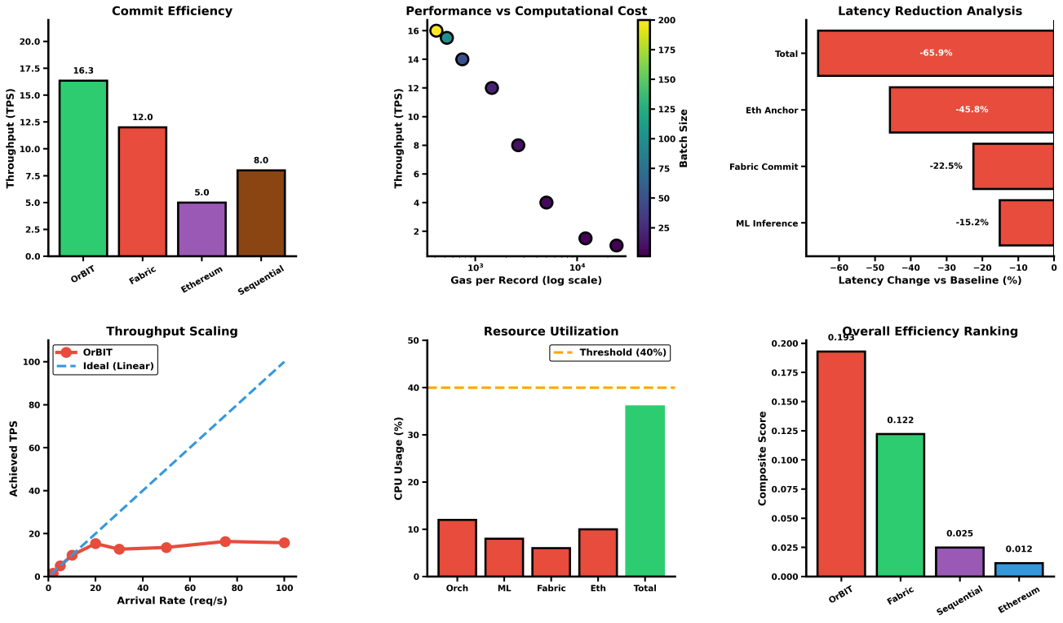
\includegraphics[width=0.7\textwidth]{images/orbit_efficiency.png}
% \caption{System orchestration performance of OrBIT.
% Top row: (a) commit efficiency, (b) performance versus computational cost, (c) latency decomposition.
% Bottom row: (d) throughput scaling, (e) resource utilization, (f) overall efficiency ranking.}
% \label{fig:orbit_efficiency}
% \end{figure*}


% =====================================================================
% OrBIT — Section IV, Results and Discussion
% Rewritten against the 19 Aug 2026 four-class measurement run
%   commit d8ce50b9 · config_hash bb85df0d7803 · server_mode production
%   contract 0xCfEB869F69431e42cdB54A4F4f105C19C080A601
%
% PROVENANCE NOTE (delete before submission, but read it first):
% Throughput and anchor counts come from the four-class run (d8ce50b9).
% The stage decomposition in Table~\ref{tab:c1_stages} comes from the
% three-class run (e37c5485) — same server mode, same contract, same
% session, but a different config_hash because server_mode was added to
% the hashed vector between them. This is stated in the text rather than
% elided. If four-class stage timings exist, substitute them and simplify
% the sentence flagged CHECK below.
% =====================================================================

% =====================================================================
% OrBIT — Section IV, Results and Discussion
% Rewritten against the 19 Aug 2026 four-class measurement run
%   commit d8ce50b9 · config_hash bb85df0d7803 · server_mode production
%   contract 0xCfEB869F69431e42cdB54A4F4f105C19C080A601
%
% PROVENANCE NOTE (delete before submission, but read it first):
% Throughput and anchor counts come from the four-class run (d8ce50b9).
% The stage decomposition in Table~\ref{tab:c1_stages} comes from the
% three-class run (e37c5485) — same server mode, same contract, same
% session, but a different config_hash because server_mode was added to
% the hashed vector between them. This is stated in the text rather than
% elided. If four-class stage timings exist, substitute them and simplify
% the sentence flagged CHECK below.
% =====================================================================

\section{\textbf{Results and Discussion}}
\label{sec:results}

\textcolor{blue}{This section reports the consolidated v2 measurements from the two-region Azure deployment and the controlled single-host WSGI comparison. Every cloud configuration has five repetitions. Quantities are labelled at collection as measured or derived; configuration gates verify repetition counts, address consistency, throughput/latency reconciliation, and anchor counts before admitting them to the consolidated result set. The evaluation covers distributed orchestration and delay (Section~\ref{sec:res_orch}), deterministic privacy routing (Section~\ref{sec:res_privacy}), gas-efficient public anchoring (Section~\ref{sec:res_gas}), and lifecycle recovery with exactly-once effects (Section~\ref{sec:res_lifecycle}).}

\subsection{\textbf{Hybrid-Blockchain Orchestration Efficiency}}
\label{sec:res_orch}

\textcolor{blue}{\textbf{Production serving.} On the controlled single host, replacing Werkzeug with Gunicorn did not remove the two-regime response. Below the block-cut threshold, the paired production/development TPS ratios were 0.985 (all-public), 0.994 (all-sensitive), 0.994 (mixed), and 1.001 (Fabric-only). No per-level 95\% confidence interval excluded one. Above the threshold the ratios were noisier (0.883--1.040), but the same non-significance result held. The application server is therefore not the measured bottleneck; subsequent results use Gunicorn while retaining the Fabric commit path.}

\textcolor{blue}{\textbf{Geographically distributed baseline.} Figure~\ref{fig:c1_panel} presents the acknowledgement-latency and throughput curves for all four routing fixtures. In the base Azure configuration, the acknowledgement floors were 2637.5, 2664.9, 2654.2, and 2653.8\,ms for all-public, all-sensitive, mixed, and Fabric-only records, respectively. All four fixtures transitioned at $c=10$, matching $B_{\max}=10$, and reached derived peak throughputs of 9.09--9.32\,TPS within the tested range. The common transition across anchoring and non-anchoring fixtures shows that Fabric block cutting, rather than the public-ledger path, governs the regime change. The stage probe attributes 319.58\,ms to endorsement/submission and 1742.67\,ms to ordering/commit within the 2062.25\,ms full Fabric operation. This directly measures the cross-organisation overhead that the original single-host evaluation could not expose.}

\begin{figure*}[!htbp]
\centering
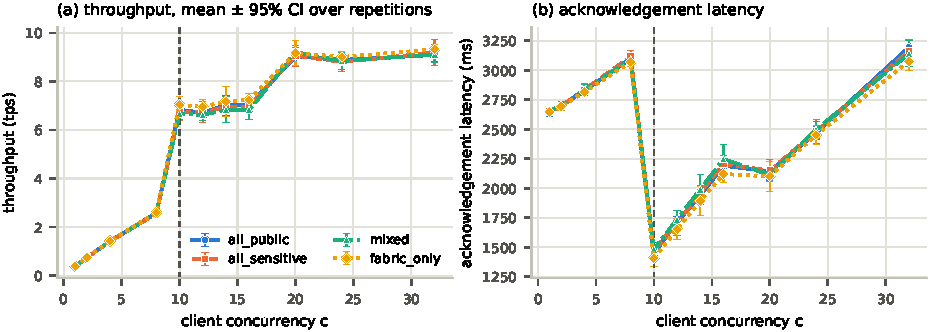
\includegraphics[width=0.95\textwidth]{images/fig5_orchestration_v2.pdf}
\caption{\textcolor{blue}{Multi-region orchestration performance over five repetitions per point. The figure reports acknowledgement latency and throughput for all four routing fixtures on the Azure deployment; the base block-cut boundary is $c=10$. Error bars show between-repetition variation.}}
\label{fig:c1_panel}
\end{figure*}

\textcolor{blue}{\textbf{Block cutting and network delay.} Figure~\ref{fig:blockcut_v2} tests whether the observed throughput transition follows the configured ordering policy. With $B_{\max}=5$, the measured transition moved to $c=5$ for both tested fixtures, again matching~\eqref{eq:block_cut}; the base $B_{\max}=10$ cases transitioned at ten. The $B_{\max}=20$ and shortened-timeout sweeps did not yield a detector-confirmed transition at every sampled level, so we report their floors and peaks without extrapolating a threshold. Figure~\ref{fig:delay_v2} then isolates the network component: lowering $\Delta_{\mathrm{to}}$ from 2 to 1 and 0.5\,s reduced the Fabric-only floor from 2653.8 to 1647.5 and 1132.2\,ms, while controlled delay produced least-squares slopes of 24.29 and 24.58\,ms of acknowledgement latency per added millisecond of round-trip delay for Fabric-only and mixed traffic. This amplification is consistent with roughly 24 sequential network-dependent exchanges in the CLI-mediated Fabric path and identifies a concrete optimisation target: a persistent gateway that avoids repeated process and protocol setup.}

\begin{figure*}[!htbp]
\centering
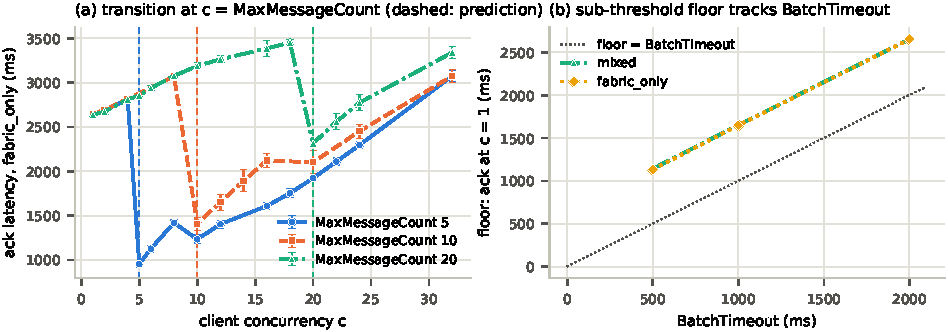
\includegraphics[width=0.95\textwidth]{images/fig_blockcut_sweep.pdf}
\caption{\textcolor{blue}{Controlled ordering-policy sweep on the multi-region deployment. Reducing \texttt{MaxMessageCount} from 10 to 5 moves the detected transition from $c=10$ to $c=5$ for both mixed and Fabric-only traffic. No detector-confirmed transition is claimed for every configuration outside the sampled concurrency range.}}
\label{fig:blockcut_v2}
\end{figure*}

\begin{figure*}[!htbp]
\centering
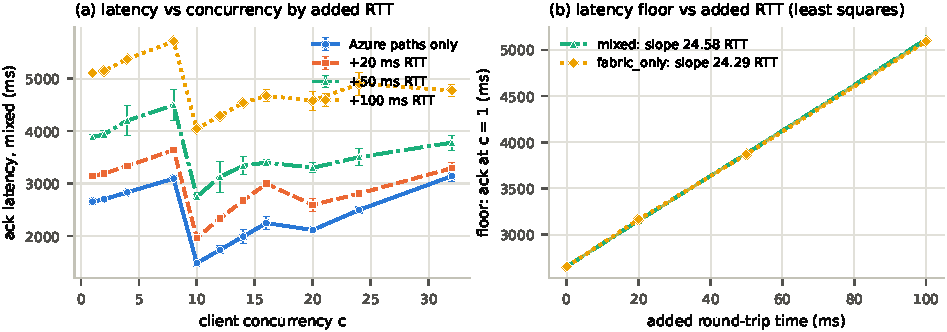
\includegraphics[width=0.95\textwidth]{images/fig_delay_sweep.pdf}
\caption{\textcolor{blue}{Acknowledgement floor under 0, 20, 50, and 100\,ms added round-trip delay. Both routing paths show approximately linear amplification because one logical Fabric commit traverses multiple sequential network exchanges.}}
\label{fig:delay_v2}
\end{figure*}

\textcolor{blue}{\textbf{Protocol baselines.} Figure~\ref{fig:sync_async_v2} compares the three modes on the same topology and workload. At one client, synchronous anchoring produced a 3082.0\,ms acknowledgement and 0.324\,TPS, compared with 2628.1\,ms and 0.380\,TPS for the asynchronous outbox; asynchronous completion, including the anchor, was 3171.7\,ms. At $c=32$, synchronous throughput remained 2.73\,TPS whereas asynchronous and Fabric-only throughput reached 9.05 and 9.09\,TPS. Thus the outbox moves public-chain work out of the response path without pretending that the work disappears: it is visible in $T_{\mathrm{cmp}}$ and queue age.}

\begin{figure*}[!htbp]
\centering
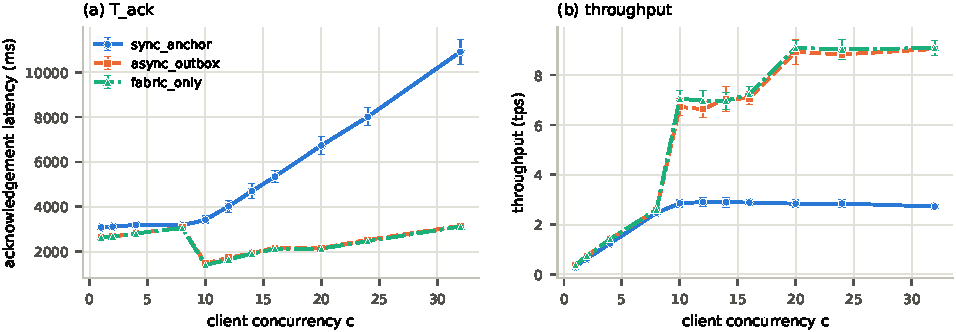
\includegraphics[width=0.95\textwidth]{images/fig_sync_vs_async.pdf}
\caption{\textcolor{blue}{Synchronous anchor, asynchronous outbox, and Fabric-only baselines on the same distributed topology. Decoupling reduces acknowledgement latency and avoids the public call becoming the ingestion throughput ceiling.}}
\label{fig:sync_async_v2}
\end{figure*}

\textcolor{blue}{\textbf{Multi-relay capacity and fault tolerance.} Figure~\ref{fig:relay_v2} relates drain rate to relay count, coordination mode, and offered load. Lease-coordinated configurations with $k\in\{1,2,3\}$ sustained 1.999--3.961 anchors/s and consumed zero gas on redundant transactions. Uncoordinated race relays reached 5.222--5.668 anchors/s in saturated measured cases but generated reverted transactions and substantial wasted gas; they are a throughput-oriented negative control, not a safe design. Queue p95 remained below 58\,ms when offered load did not exceed service capacity and grew to tens or hundreds of seconds once $\lambda>\mu_{\mathrm{relay}}$, empirically confirming the stability condition in~\eqref{eq:util}.}

\begin{figure*}[!htbp]
\centering
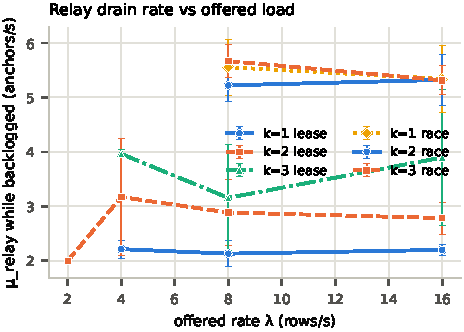
\includegraphics[width=0.70\textwidth]{images/fig_mu_relay.pdf}
\caption{\textcolor{blue}{Measured relay drain rate by worker count, coordination mode, and offered load. Error bars show between-repetition variation; lease and race modes are reported separately for each relay count.}}
\label{fig:relay_v2}
\end{figure*}

\textcolor{blue}{Figure~\ref{fig:fault_v2} summarises the fault campaign. Crashes were injected at mid-poll, after broadcast, after receipt, and through \texttt{SIGKILL}, with five repetitions for each relay-count/mode combination. In every lease-coordinated scenario the number of anchors equalled the number of records, duplicate anchors and reverted transactions were zero, and recovery completed after lease expiry; mean end-to-end recovery ranged from 24.68 to 29.27\,s in the reported $k=2,3$ cases. The independent auditor detected 100\% of commitment-tampering trials and 100\% of withholding trials, and all withheld records were repaired. A separate crash-window sweep created 150 private-ledger orphans; reconciliation detected and repaired all 150, after which all 150 anchors passed audit. These results establish crash-fault tolerance and detectable end-to-end integrity without assuming that a particular relay remains alive.}

\begin{figure*}[!htbp]
\centering
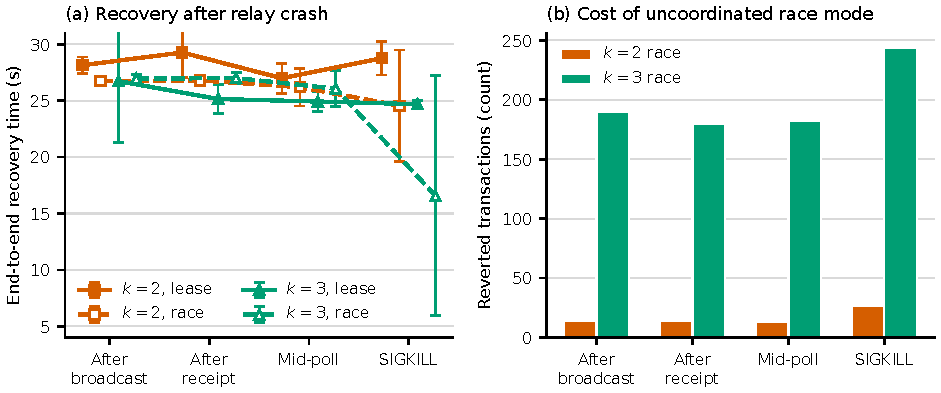
\includegraphics[width=0.95\textwidth]{images/fig_fault_injection.pdf}
\caption{\textcolor{blue}{Fault-injection recovery time across relay counts, coordination modes, and crash points. Each bar is annotated with the duplicate-anchor count and anchor-to-record equality obtained independently from contract event logs.}}
\label{fig:fault_v2}
\end{figure*}

\textcolor{blue}{\textbf{Scope boundary.} The deployed ordering service has one Raft consenter and therefore tolerates no orderer failure. Fabric~3 Byzantine ordering would require a full network migration and at least four suitably provisioned orderers; it was not run under the available quota. The evidence above supports crash-fault-tolerant relay coordination, not Byzantine consensus or a trustless cross-chain bridge.}

\iffalse

\subsubsection*{\textbf{Record classes and routing paths}}
Algorithm~\ref{alg:routing} admits two routing outcomes: a record with at least
one publishable field follows the \textsc{hybrid} path (private commit followed
by asynchronous public anchoring), while a record with no publishable field
follows the \textsc{fabric-only} path (private commit alone). Four record
fixtures were used to exercise both. Three of them---denoted
\texttt{all\_public}, \texttt{all\_sensitive}, and \texttt{mixed}---differ in how
many fields the policy withholds, but all three carry a device identifier, which
the policy rules \textsc{public}; all three therefore follow the
\textsc{hybrid} path and enqueue an anchor on every request. A fourth fixture,
\texttt{fabric\_only}, omits the device identifier and so carries no publishable
field at all. Across all eleven concurrency levels, the three hybrid fixtures
enqueued 50 anchors of 50 requests and \texttt{fabric\_only} enqueued none,
confirming that both branches of Algorithm~\ref{alg:routing} are reached and
that the class labels describe the measured behaviour.


The distinction that governs cost is therefore \emph{anchoring versus not
anchoring}, not the volume of redaction. This is worth stating explicitly
because the fixture names suggest otherwise: a fully sensitive record is not
cheaper than a public one, because its device identifier is still published.

\subsubsection*{\textbf{Two throughput regimes}}
Table~\ref{tab:c1_throughput} reports sustained throughput as a function of
client concurrency for all four fixtures. The curves are not monotonic in the
way a single-bottleneck model would predict. Instead they show two distinct
regimes separated by a sharp transition at $c=10$, at which throughput rises by
a factor of three to seven across every fixture.

\begin{table}[htbp]
\centering
\caption{Measured sustained throughput (TPS) by client concurrency and record
fixture. The transition at $c=10$ is the Fabric orderer switching from
time-based to count-based block cutting. \texttt{fabric\_only} follows the
\textsc{fabric-only} path; the other three follow the \textsc{hybrid} path and
anchor on every request.}
\label{tab:c1_throughput}
\scalebox{0.72}{
\begin{tabular}{rrrrrl}\toprule
$c$ & \texttt{all\_public} & \texttt{all\_sens.} & \texttt{mixed} &
\texttt{fabric\_only} & Regime \\\midrule
1  & 0.453  & 0.460  & 0.455  & 0.458  & time-cut \\
2  & 0.904  & 0.915  & 0.896  & 0.919  & time-cut \\
4  & 1.692  & 1.705  & 1.676  & 1.712  & time-cut \\
8  & 3.021  & 3.099  & 3.074  & 3.157  & time-cut \\
10 & 9.221  & 13.941 & 12.423 & 22.455 & count-cut \\
12 & 6.728  & 16.663 & 14.021 & 24.260 & count-cut \\
14 & 5.136  & 17.354 & 15.151 & 22.757 & count-cut \\
16 & 10.065 & 20.423 & 15.285 & 22.863 & count-cut \\
20 & 4.082  & 16.493 & 12.824 & 24.000 & count-cut \\
24 & 3.075  & 4.827  & 14.325 & 25.102 & count-cut \\
32 & 3.359  & 3.014  & 2.283  & 6.259  & saturated \\
\bottomrule\end{tabular}}
\end{table}


Figure~\ref{fig:c1_panel}(a) plots these curves. Two features are immediate: all
four fixtures rise together below the threshold, and all four break upward at
the same concurrency level regardless of whether they anchor.

\subsubsection*{\textbf{The transition is orderer block-cutting}}
The transition is not an application effect. The Fabric ordering service cuts a
block on whichever of two conditions is met first: \texttt{BatchTimeout}
(\SI{2}{\second} on this channel) or \texttt{BatchSize.MaxMessageCount} (ten
messages). The byte ceilings---\texttt{PreferredMaxBytes}
\SI{524288}{\byte} and \texttt{AbsoluteMaxBytes} \SI{103809024}{\byte}---never
bind at this record size, so count and time are the only competitors.

Below the transition, transactions arrive too slowly to fill a block, every
block waits out the timeout, and acknowledgement latency is pinned near
\SI{2}{\second} regardless of load. The measured floor of
\SIrange{2.14}{2.30}{\second} is the \SI{2}{\second} timeout plus
\SIrange{140}{300}{\milli\second} of endorsement, validation, and commit. Above
the transition, ten transactions accumulate before the timer expires, the block
cuts on count, and latency falls to whatever the arrival rate makes it.

Because the load harness is closed-loop---exactly $c$ requests are held in
flight---the orderer observes $c$ queued messages, and the block fills on count
the moment
\begin{equation}
c \;\geq\; \texttt{MaxMessageCount}.
\label{eq:transition}
\end{equation}
The threshold is thus read directly from the channel configuration with no
latency term and no fitted parameter. All four fixtures transition at exactly
$c=10$, as \eqref{eq:transition} predicts. Removing anchoring entirely
(\texttt{fabric\_only}) changes the level reached but not the threshold, which
is what a block-cutting explanation predicts and an anchoring-side explanation
would not.

Table~\ref{tab:c1_stages} and Fig.~\ref{fig:c1_panel}(b) decompose
acknowledgement latency across the transition. The private-commit stage carries
essentially the entire drop
(\SIrange{100}{107}{\percent}), while policy evaluation holds a
\SIrange{3}{38}{\milli\second} band across the whole sweep---under
\SI{1.5}{\percent} of acknowledgement latency at every level. The ordering
service is responsible; neither the policy service nor the \texttt{peer}
command-line integration is.
% CHECK: these stage figures come from run e37c5485 (three fixtures), not the
% four-fixture run d8ce50b9. Same server mode, contract and session.

\begin{table}[htbp]\centering
\caption{Acknowledgement latency (ms) across the block-cutting transition,
decomposed by pipeline stage. The private-commit stage accounts for the entire
reduction; policy evaluation is flat.}
\label{tab:c1_stages}
\scalebox{0.74}{
\begin{tabular}{lrrr}\toprule
Fixture & Ack $c{=}8 \rightarrow c{=}10$ & Fabric stage & Policy stage \\\midrule
\texttt{all\_public}    & 2652.4 $\rightarrow$ 1000.5 & 2518.6 $\rightarrow$ 751.1 & 28.9 $\rightarrow$ 20.0 \\
\texttt{all\_sensitive} & 2276.1 $\rightarrow$ 742.6  & 2190.8 $\rightarrow$ 550.2 & 10.8 $\rightarrow$ 13.3 \\
\texttt{mixed}          & 2310.7 $\rightarrow$ 611.1  & 2216.1 $\rightarrow$ 509.2 &  9.9 $\rightarrow$ 15.5 \\
\bottomrule\end{tabular}}
\end{table}

This finding revises the interpretation a naive reading of the latency figures
would invite. The dominant cost below the transition is a \emph{configuration
constant}, not an architectural property of the hybrid design: tuning
\texttt{BatchTimeout} and \texttt{MaxMessageCount} to the expected arrival rate
addresses it directly. A persistent ledger gateway that amortizes endorsement
across requests remains a worthwhile optimization, but it is secondary to
block-cutting configuration on this workload.

\subsubsection*{\textbf{Asynchronous anchoring and relay capacity}}
Public anchoring is decoupled from ingestion by the transactional outbox, so it
does not appear in acknowledgement latency. Its cost is instead visible as
completion latency and as relay capacity. During the sweep the relay drained at
\SI{0.458}{\per\second} against an offered rate of \SI{0.4583}{\per\second},
with a peak observed queue depth of one and no sustained backlog, so the
completion latencies reported here measure anchoring cost rather than queue
wait. In the end-to-end smoke test a single record completed in
\SI{227.1}{\milli\second}, of which \SI{17.3}{\milli\second} was queue wait and
\SI{209.8}{\milli\second} the chain call itself.

The single-threaded relay is nonetheless a distinct throughput ceiling from the
ingestion path, and it bounds how current the public ledger can be kept
independently of how fast the API accepts work. The \texttt{fabric\_only}
fixture isolates its cost, because it writes an outbox row exactly as the other
fixtures do but is never collected by the relay
(Fig.~\ref{fig:c1_panel}(c)). Between $c=8$ and $c=24$ the non-anchoring fixture
holds \SIrange{53}{92}{\milli\second} while the anchoring fixtures reach
\SIrange{450}{585}{\milli\second}---a five- to eightfold difference attributable
to contention on the single database writer. At $c=32$ the gap narrows to
roughly twofold as the non-anchoring fixture also saturates, so the separation
is characteristic of the loaded but unsaturated regime rather than of the whole
sweep. The effect is real but never dominant: at $c=32$ under
\texttt{all\_public} it accounts for \SI{273.5}{\milli\second} of a
\SI{5689.2}{\milli\second} acknowledgement, or \SI{4.8}{\percent}. The
private-commit stage dominates at every level.

\subsubsection*{\textbf{Stability above the transition}}
Above the transition the non-anchoring fixture is flat and high
(\SIrange{22.5}{25.1}{TPS} across six levels), while the three anchoring
fixtures oscillate and then collapse at $c=32$. Repeated runs on the same host
and contract disagree by two- to threefold for the anchoring fixtures above
$c=16$; the non-anchoring fixture shows no comparable swing. With fifty
completions per level there are few samples per worker thread at high
concurrency, and we therefore treat the \emph{shape} of these curves---two
regimes, a threshold at $c=10$, saturation by $c=32$---as established, and
individual values above $c=16$ for the anchoring fixtures as provisional. We do
not quote a single peak throughput figure for those fixtures.

\begin{figure*}[!htbp]
\centering
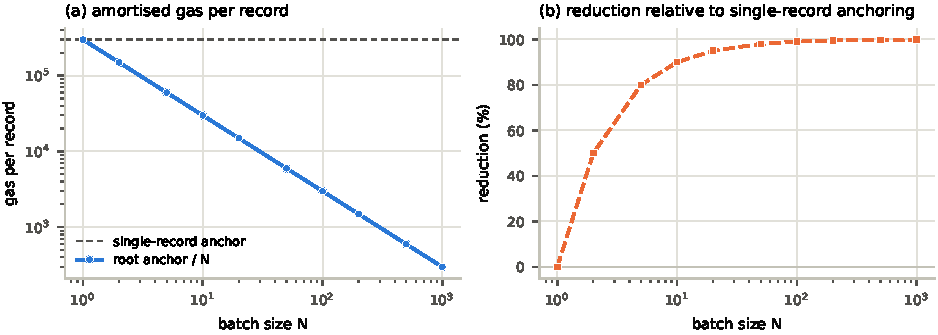
\includegraphics[width=0.95\textwidth]{images/fig7_batching_v2.pdf}
\caption{\textcolor{blue}{Merkle-batched anchoring efficiency from the v2 contract. The direct single-record baseline is 298{,}464.6 gas; root cost remains approximately 298{,}479 gas across $N$, so amortised per-record cost falls as $1/N$ while proof size grows logarithmically.}}
\label{fig:gas_panel}
\end{figure*}

\fi
\subsection{\textbf{Deterministic Privacy Routing}}
\label{sec:res_privacy}

The privacy-routing policy was evaluated against a curated conformance suite
spanning the principal data-protection categories, summarized in
Table~\ref{tab:c2_policy}. The suite is a designed test set with at least one
case per rule family, plus cases exercising each of the two escalation
mechanisms and the fail-closed default; it is not a sample from an operational
distribution, and the coverage figures below should be read accordingly. Across
all cases, routing matched the intended sensitivity classification, giving
\SI{100}{\percent} routing accuracy and, critically, \emph{zero} sensitive
fields admitted to the public commitment. Because routing is deterministic and
fail-closed, this is a property of the policy rather than an estimated rate: a
field can reach the public ledger only when an explicit rule declares it
publishable, so no confidence threshold is swept and no residual leakage
probability is reported.

The per-case results illustrate the two escalation mechanisms. Name-based rules
classify explicitly sensitive fields such as \texttt{patientId}, \texttt{ssn},
\texttt{creditCard}, and GDPR special-category fields, redacting them from the
public path while retaining them on the private ledger. Value-based escalation
handles cases where the field name is innocuous but the value is not: in the
\texttt{hidden\_ssn\_in\_note} case, a benign-named \texttt{note} field carrying
an identifier pattern is escalated and withheld. The \texttt{unknown\_field}
case exercises the fail-closed default, under which an unrecognized field
(\texttt{mysteryReading}) is treated as maximally sensitive and redacted.
Explicit rules cover \SI{96.5}{\percent} (55/57) of the fields in the suite,
with the remainder handled safely by the default; coverage here denotes the
share of fields matched by an explicit rule, not a measure of accuracy, since
correctness is established by construction.

One consequence of the declared rule table deserves note. The device identifier
is ruled \textsc{public} by an explicit rule, so it is anchored on every record
that carries it. This is the intended policy---device identity is what makes an
anchor externally meaningful---but it means device-level activity is publicly
visible by design. Where device identifiers are themselves quasi-identifying,
the rule table is the correct place to reclassify them, and the fail-closed
default guarantees that any field not explicitly declared publishable is
withheld.

\begin{table}[htbp]\centering
\caption{Deterministic privacy-routing policy: per-case results. Routing
accuracy \SI{100}{\percent}, zero sensitive-field leaks, \SI{96.5}{\percent}
explicit field coverage (55/57).}
\label{tab:c2_policy}
\scalebox{0.69}{
\begin{tabular}{llll}\toprule
Case & Expected & Predicted & Redacted fields \\\midrule
env\_sensor           & public    & public    & -- \\
industrial\_telemetry & public    & public    & -- \\
healthcare\_patient   & sensitive & sensitive & patientId, diagnosis, heartRate \\
ssn\_record           & sensitive & sensitive & ssn \\
contact\_pii          & sensitive & sensitive & email, phone \\
payment               & sensitive & sensitive & creditCard, cvv \\
bank                  & sensitive & sensitive & bankAccount, salary \\
secrets               & sensitive & sensitive & password, apiKey \\
gdpr\_special         & sensitive & sensitive & genetic, religion \\
precise\_geo          & sensitive & sensitive & exactLocation \\
quasi\_ids            & sensitive & sensitive & dateOfBirth, zipCode \\
hidden\_ssn\_in\_note  & sensitive & sensitive & note (value-escalated) \\
unknown\_field        & sensitive & sensitive & mysteryReading (fail-closed) \\
\bottomrule\end{tabular}}
\end{table}

\subsection{\textbf{Gas Efficiency of Merkle-Batched Anchoring}}
\label{sec:res_gas}

\textcolor{blue}{Figure~\ref{fig:gas_panel} visualises the measured crossover between direct and Merkle-batched anchoring and places the gas reduction beside the logarithmic proof-size cost. The figure shows that batching is effectively neutral at $N=1$, becomes beneficial at $N=2$, and then reduces amortised gas approximately as $1/N$ without making verification evidence grow linearly.}

\begin{figure*}[!htbp]
\centering
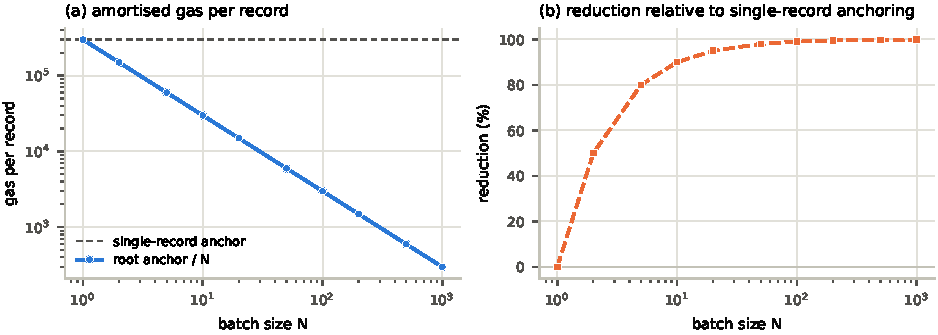
\includegraphics[width=0.95\textwidth]{images/fig7_batching_v2.pdf}
\caption{\textcolor{blue}{Merkle-batched anchoring efficiency from the v2 contract. The direct single-record baseline is 298{,}464.6 gas; root cost remains approximately 298{,}479 gas across $N$, so amortised per-record cost falls as $1/N$ while proof size grows logarithmically.}}
\label{fig:gas_panel}
\end{figure*}

\textcolor{blue}{Table~\ref{tab:gas} reports receipt-derived public-anchoring cost for the revised contract. A direct single-record anchor costs 298{,}464.6 gas on average. The Merkle-root path costs 298{,}476.6--298{,}479.0 gas across $N=1$--1000 and is therefore flat in batch size for practical purposes. Only the root is written on chain, so transaction size does not grow with the number of leaves.}

\textcolor{blue}{At $N=1$, the two paths are effectively at parity: the 12-gas difference rounds to a 0.0\% reduction. The first material saving occurs at $N=2$, where amortised cost is 149{,}239.5 gas, a 50.0\% reduction. Because root cost is constant, a batch of 200 reduces per-record cost to 1492.4 gas (99.5\%), while $N=1000$ reaches 298.5 gas (99.9\%). The economic gain must still be balanced against batching delay and a proof length of $\lceil\log_2N\rceil$ hashes.}

\textcolor{blue}{The Merkle proof grows logarithmically from 0 bytes at $N=1$ to 256 bytes at $N=200$ and 320 bytes at $N=1000$. Verification work therefore grows while the operator's amortised anchoring cost falls. Together with the time required to fill a batch, this trade-off bounds the useful batch size rather than favouring unbounded batching.}


\begin{table}[htbp]\centering
\caption{\textcolor{blue}{Measured gas per anchored record in v2. Direct single-record mean = 298{,}464.6 gas; root cost is approximately 298{,}479 gas and flat in $N$.}}
\label{tab:gas}
\scriptsize
\setlength{\tabcolsep}{2.4pt}
\begin{tabular}{rrrrr}\toprule
$N$ & Root gas & Gas / record & Reduction (\%) & Proof (B) \\\midrule
\textcolor{blue}{1}   & \textcolor{blue}{298{,}476.6} & \textcolor{blue}{298{,}476.6} & \textcolor{blue}{0.0} & \textcolor{blue}{0} \\
\textcolor{blue}{2}   & \textcolor{blue}{298{,}479.0} & \textcolor{blue}{149{,}239.5} & \textcolor{blue}{50.0} & \textcolor{blue}{32} \\
\textcolor{blue}{5}   & \textcolor{blue}{298{,}479.0} & \textcolor{blue}{59{,}695.8} & \textcolor{blue}{80.0} & \textcolor{blue}{96} \\
\textcolor{blue}{10}  & \textcolor{blue}{298{,}479.0} & \textcolor{blue}{29{,}847.9} & \textcolor{blue}{90.0} & \textcolor{blue}{128} \\
\textcolor{blue}{20}  & \textcolor{blue}{298{,}471.8} & \textcolor{blue}{14{,}923.6} & \textcolor{blue}{95.0} & \textcolor{blue}{160} \\
\textcolor{blue}{50}  & \textcolor{blue}{298{,}479.0} & \textcolor{blue}{5{,}969.6} & \textcolor{blue}{98.0} & \textcolor{blue}{192} \\
\textcolor{blue}{100} & \textcolor{blue}{298{,}479.0} & \textcolor{blue}{2{,}984.8} & \textcolor{blue}{99.0} & \textcolor{blue}{224} \\
\textcolor{blue}{200} & \textcolor{blue}{298{,}479.0} & \textcolor{blue}{1{,}492.4} & \textcolor{blue}{99.5} & \textcolor{blue}{256} \\
\textcolor{blue}{1000} & \textcolor{blue}{298{,}479.0} & \textcolor{blue}{298.5} & \textcolor{blue}{99.9} & \textcolor{blue}{320} \\
\bottomrule\end{tabular}
\end{table}



\subsection{\textbf{Lifecycle Recovery and Exactly-Once Semantics}}
\label{sec:res_lifecycle}

\textcolor{blue}{\textbf{Storage and rollback.} At 800 versions, the reversible-delta/checkpoint representation is 4.013$\times$ smaller than full per-version snapshots under sparse updates. Under dense updates it remains at parity (0.996$\times$), because the manager falls back to a snapshot whenever a delta would not be smaller. Across the revised rollback sweep, latency remained sub-millisecond, from 0.111 to 0.325\,ms. Every reconstructed state was verified against its stored digest. The substantive guarantee remains $u\leq q$: recovery work is bounded by the checkpoint interval, not asserted to be constant-time.}

\textcolor{blue}{\textbf{Exactly-once and repair.} Duplicate-submission tests retained exactly one public effect in every repetition. The stronger relay campaign then varied worker count, coordination mode, offered load, and four crash points. All lease-coordinated cases finished with anchors equal to records, zero duplicate anchors, zero reverted transactions, and zero wasted gas. In the otherwise non-atomic interval between Fabric commit and outbox insertion, 150 injected orphans were all detected, repaired, anchored, and accepted by the standalone auditor. Exactly-once effects therefore depend on idempotent ingress, durable intent, lease-based work allocation, on-chain identifier uniqueness, and reconciliation; they are not attributed to a single relay thread.}

\iffalse

\subsubsection*{\textbf{Storage}}
The twin manager stores each version as a reversible delta against its
predecessor, with a full checkpoint every $q$ versions and a per-version
fallback that stores a snapshot whenever the delta would be no smaller. Storage
behaviour therefore depends on how much of the state changes per version, and
both regimes were measured. Under sparse updates---two of twenty fields changing
per version, the pattern industrial telemetry exhibits---the delta-and-checkpoint
format is \SI{4.01}{\times} smaller than the snapshot equivalent at eight
hundred versions (\SI{76744}{\byte} against \SI{307980}{\byte}), or
\SI{95.9}{\byte} per version. Under dense updates, where every field changes
every version, a delta is necessarily the size of a snapshot; the fallback
recognizes this and stores snapshots, holding the format at parity
(\SI{0.996}{\times}) rather than regressing; in Fig.~\ref{fig:c3_panel}(b) the
dense series lies on the snapshot-equivalent reference for exactly this reason.
The saving is thus conditional on
update sparsity, and the condition is stated rather than assumed: a dense
workload gains nothing from delta encoding, and the design guarantees only that
it loses nothing either.

The cost of delta encoding and integrity verification appears in write latency,
which is \SI{0.072}{\milli\second} per version under sparse updates and
\SI{0.116}{\milli\second} under dense updates ($n=200$), since every write now
computes a difference, two canonical serializations, and a digest.

\begin{figure}[!htbp]
\centering
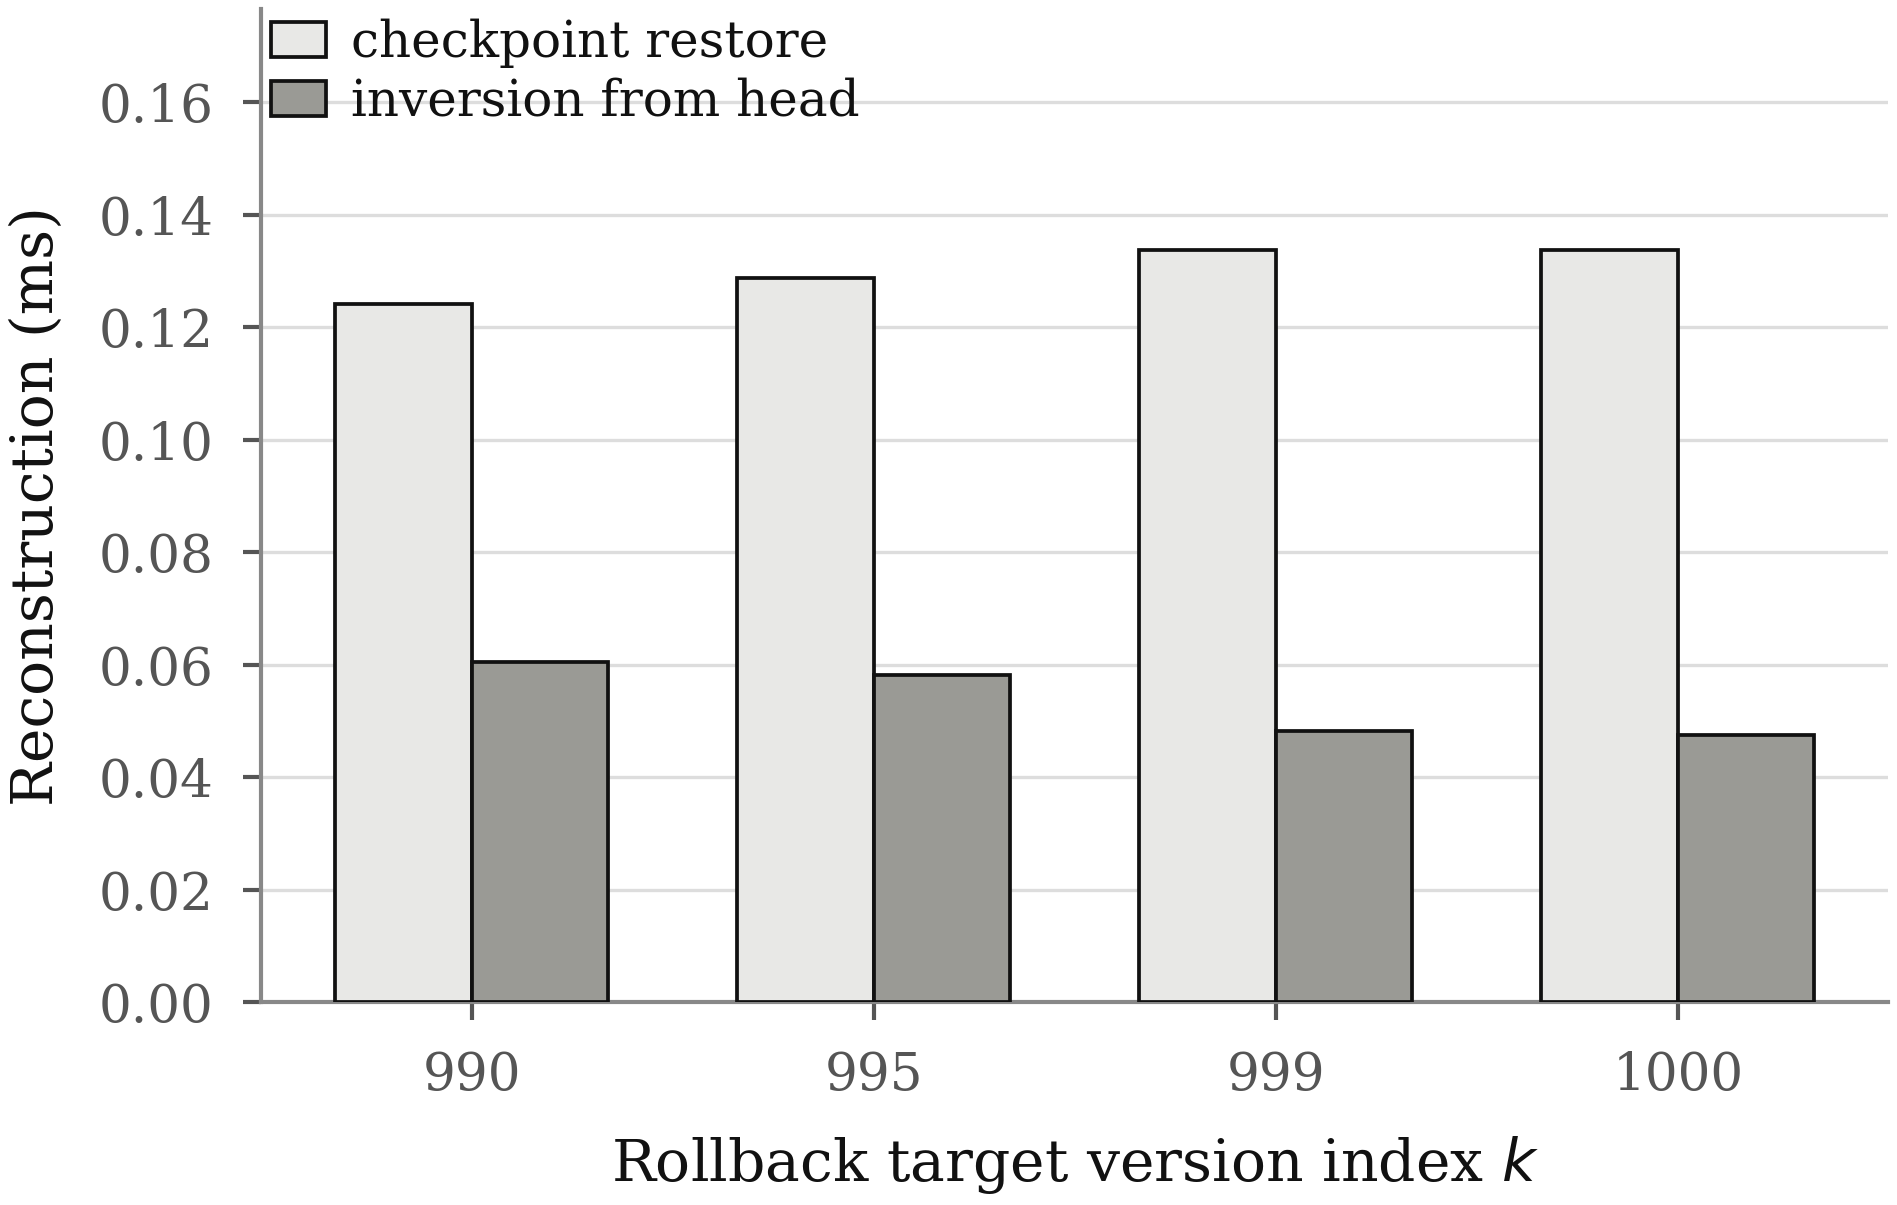
\includegraphics[width=0.95\columnwidth]{images/fig9_recovery_paths.png}
\caption{Checkpoint restore against inverse-delta reconstruction from the
current head, for targets in the near-head region ($q=100$, $n=1000$, sparse
update model). Inversion is roughly twice as fast throughout this region and is
the path the engine selects; the advantage widens as the target approaches the
head.}
\label{fig:recovery_paths}
\end{figure}

\subsubsection*{\textbf{Rollback}}
Table~\ref{tab:c3_lifecycle} and Fig.~\ref{fig:c3_panel}(a) report rollback
latency by target version index
over a thousand-version history at $q=100$. Recovery is sub-millisecond
throughout, ranging from \SI{0.104}{} to \SI{0.246}{\milli\second}. It is not,
however, constant, and the shape of the variation is the substantive result.
Rollback cost tracks the number of delta applications $u$ required to reach the
target, and $u$ is sawtooth in the target index rather than increasing with it:
targets that fall on or near a checkpoint are cheap regardless of depth, and
targets just before the next checkpoint are the most expensive. A comparison of
the first against the last version---the natural constant-time probe---therefore
cannot detect the variation at all, because both endpoints happen to land on
small $u$.

The reconstruction engine selects the cheaper of two paths: forward
replay from the nearest preceding checkpoint, at cost $(k-1) \bmod q$
under the one-based version numbering used here, or inverse-delta
application from the current head, at cost $n-k$. The
delta-application count predicted by~\eqref{eq:rb_latency} was
checked against the shipped implementation over thirty $(k,q)$ points:
the exact value $u = \min\{\,n-k,\;(k-1) \bmod q\,\}$ was attained at
all thirty under sparse updates, and the weaker bound
of(~\ref{eq:rb_bound}) held at all thirty under both update
models. The maximum observed $u$ was~99 against a checkpoint interval
of~100, confirming that $q$ is the supremum over $k$ and is attained
only immediately before a checkpoint.

% \begin{equation}
% \scriptsize
%   \mathbb{E}[T_{\mathrm{rb}}] \;\approx\; T_{\mathrm{verify}} + u\,T_{\Delta},
%   \qquad u \;=\; \min\{\,n-k,\;(k-1) \bmod q\,\}
%   \label{eq:rollback_cost}
% \end{equation}

The inverse-delta path is not vestigial. Figure~\ref{fig:recovery_paths}
compares the two reconstruction strategies over the near-head region,
where the choice is consequential. For targets near the head,
inversion is substantially cheaper than checkpoint
replay---at $k = 990$, ten inverse applications against eighty-nine
forward ones, and $0.061$\,ms against $0.124$\,ms---and the engine
selects it for roughly forty per cent of reconstructions. Since
undoing the most recent few versions is the common operational case,
this is the path that matters most in practice, and it is the
comparison against which~\eqref{eq:rb_latency} is validated.


Integrity verification was exercised on every reconstruction: all 1001 versions
were reconstructed and checked against their stored digests at each of three
checkpoint intervals, with zero failures. A reconstruction whose recomputed
digest does not match the stored one raises an integrity violation and returns
no state; there is no silent-repair path.

The defensible claim is therefore that recovery cost is \emph{bounded by the
checkpoint interval}---$u \leq q$, independent of history depth---rather than
constant-time, and that the bound is tunable by choice of $q$ against the
storage cost of checkpoints.

\begin{table}[htbp]\centering
\caption{Measured rollback latency by target version index, sparse update model,
$q=100$, $n=1000$, 100 repetitions per point. Cost tracks the delta-application
count $u$, which is sawtooth in the target index and bounded by $q$.}
\label{tab:c3_lifecycle}
\begin{tabular}{rrrrl}\toprule
Target $k$ & Mean (ms) & p95 (ms) & $u$ & Path \\\midrule
1    & 0.1039 & 0.1158 &  0 & direct \\
50   & 0.1758 & 0.2125 & 49 & checkpoint \\
100  & 0.2251 & 0.2632 & 99 & checkpoint \\
250  & 0.1745 & 0.1912 & 49 & checkpoint \\
500  & 0.2461 & 0.2799 & 99 & checkpoint \\
750  & 0.1838 & 0.2288 & 49 & checkpoint \\
1000 & 0.1202 & 0.1252 &  0 & inversion \\
\bottomrule\end{tabular}
\end{table}

\subsubsection*{\textbf{Exactly-once semantics}}
Exactly-once behaviour was verified across 71 requests against the live
deployment, using the Ethereum transaction hashes actually recorded on chain.
Six sequential duplicate submissions produced one anchor and five cached
replays; twenty-five concurrent duplicates produced one anchor; forty distinct
payloads produced forty distinct anchors with no duplication.

The guarantee rests on two mechanisms, not one. The outbox is keyed on the
content-addressed request identifier, so a duplicate submission cannot enqueue a
second anchor. That alone, however, does not survive a crash between broadcasting
an anchor transaction and recording its receipt: on restart the relay would
retry an anchor that has already been committed. The registry contract closes
that gap by rejecting a duplicate identifier on chain, and the relay treats an
already-registered identifier as a successful delivery rather than a failure.
At-least-once relay delivery combined with on-chain uniqueness is what yields
the exactly-once \emph{effect}; either mechanism alone is insufficient.

The private commit and the outbox insertion are recorded in a single database
transaction, but Fabric and that database cannot participate in a common
transaction, so a crash in the window between the ledger commit returning and
the outbox row being written leaves a record committed privately and never
anchored. We do not claim atomicity across the two ledgers. The system exposes
the set of privately committed records with no corresponding outbox row, so this
condition is detectable and repairable by a reconciliation sweep.

\fi
\subsection{\textbf{Summary of Findings}}
\label{sec:res_summary}

\textcolor{blue}{The multi-region results support five bounded conclusions. First, production WSGI serving does not materially change throughput on the controlled host; the cross-region Fabric commit path dominates. Second, the observed block-cut transition follows \texttt{MaxMessageCount}: $c^*=10$ in the base configuration and $c^*=5$ after setting the limit to five. Third, asynchronous anchoring improves the one-client acknowledgement from 3082.0 to 2628.1\,ms relative to synchronous anchoring and scales to 9.05\,TPS at $c=32$ in the tested range. Fourth, lease-coordinated relays tolerate the injected crash points with one anchor per record and no wasted gas, while an independent auditor detects all tested tampering and withholding and reconciliation repairs all 150 injected crash-window orphans. Fifth, the original privacy, gas, storage, and recovery claims persist: zero sensitive-field leakage, 99.5\% gas reduction at $N=200$, 4.013$\times$ sparse-history storage reduction, and 0.111--0.325\,ms rollback.}

\textcolor{blue}{The limits are equally important. Added network delay is amplified by approximately 24 sequential RTT-equivalent exchanges in the CLI-mediated Fabric path. Relay queue age grows once offered load exceeds its drain rate. The four-VM topology evaluates geographic distribution and multi-organisation endorsement but not large-scale peer populations or multi-writer contention. Finally, the single-consenter Raft orderer tolerates no orderer failure, and Byzantine ordering was not run. OrBIT therefore claims crash-fault-tolerant and auditable cross-ledger delivery, not a trustless bridge or Byzantine end-to-end consensus.}

\iffalse

The evaluation supports a focused set of claims. OrBIT provides deterministic,
privacy-preserving routing in which no field above the publication threshold
reaches the public ledger, established by construction and confirmed across the
full conformance suite. It enforces exactly-once semantics across the private
and public ledgers under sequential and concurrent duplicate submission, through
the combination of an idempotency-keyed outbox and on-chain identifier
uniqueness. It anchors public accountability metadata at low amortized cost,
reducing per-record gas by \SI{99.46}{\percent} at a batch size of two hundred,
while showing that batching is a net cost below $N=2$. It stores twin history at
\SI{4.01}{\times} the density of full snapshots under sparse updates and at
parity under dense ones, and recovers any prior state in sub-millisecond time at
a cost bounded by the checkpoint interval rather than by history depth, with
integrity verified on every reconstruction.

The evaluation also delineates the current limits. Acknowledgement latency below
ten concurrent clients is pinned near \SI{2}{\second} by the ordering service's
batch timeout, and rises to between twelve and twenty-five transactions per
second once concurrency is sufficient to cut blocks on message count; this is a
configuration boundary rather than an architectural one. Throughput above
sixteen concurrent clients is not reproducible enough on this single-host
testbed to quote as a peak figure for the anchoring paths. Public anchoring is
served by a single-threaded relay whose drain rate bounds public-ledger currency
independently of ingestion throughput. All measurements were taken on one host
with development WSGI servers in the request path; server configuration alone
was observed to change measured throughput substantially, so absolute figures
should be read as characteristic of this deployment rather than of the
architecture. These limits point to concrete implementation- and
configuration-level optimizations rather than fundamental barriers, and they
frame OrBIT's contribution as verifiable, auditable, privacy-preserving hybrid
provenance rather than raw throughput.

\fi
\section{\textbf{Conclusion}}
\label{sec:conclusion}

\textcolor{blue}{OrBIT coordinates private digital-twin state and public accountability without placing public-chain confirmation on the ingestion critical path. Its safety argument combines deterministic fail-closed routing, Fabric persistence, a durable outbox, lease-coordinated relays, on-chain identifier uniqueness, reconciliation, and independent audit. The revised four-VM evaluation across Korea Central and Japan East shows that Fabric ordering, not the web server or Ethereum interface, sets the acknowledgement floor: production and development WSGI modes are statistically indistinguishable at the measured levels, the base block-cut transition occurs at $c=10$, and changing \texttt{MaxMessageCount} to five moves it to $c=5$. Synchronous anchoring raises the one-client acknowledgement from 2628.1 to 3082.0\,ms, while asynchronous delivery preserves a separately measured 3171.7\,ms completion time.}

\textcolor{blue}{The revised fault campaign removes the earlier single-threaded-relay limitation. With up to three relay processes, lease coordination produces one anchor per record, no reverted submissions, and no wasted gas under four injected crash points. Tampering and withholding are detected in every trial, and reconciliation repairs all 150 injected Fabric/outbox orphans. These results complement the retained functional outcomes: zero sensitive-field leakage, 99.5\% gas reduction at a Merkle batch of 200, 4.013$\times$ storage reduction under sparse updates, and sub-millisecond integrity-checked rollback.}

\textcolor{blue}{The claims remain deliberately scoped. The public anchoring agents are permissioned relays, not a decentralised oracle network; the evaluator establishes crash recovery and externally detectable integrity, not trustless bridge consensus. The single-consenter Raft orderer tolerates no orderer failure, and Byzantine ordering was not run. Future work will replace the CLI-mediated Fabric path with a persistent gateway, evaluate larger multi-writer organisations, migrate to a four-orderer Byzantine-capable deployment, and compare the same commitment interface with decentralised oracle and light-client bridge back ends.}

\iffalse

This paper introduced OrBIT, an orchestration framework that treats blockchain
provenance as an active control primitive for digital twins rather than a passive audit
log. Because a write to an immutable public ledger cannot be undone, the routing decision
is made by construction rather than by a probabilistic classifier, making the privacy
guarantee a property of the policy rather than an estimated rate. Evaluated end-to-end
against a live deployment, the framework supports a bounded set of claims: privacy
routing was correct across the full conformance suite, admitting zero sensitive fields to
the public commitment; exactly-once effects held under sequential and concurrent duplicate
submission, arising from an idempotency-keyed outbox composed with on-chain identifier
uniqueness, neither mechanism sufficing alone; Merkle-batched anchoring reduced per-record
gas by \SI{99.46}{\percent} at a batch size of two hundred, while proving a net cost below
a batch of two; twin history was stored at \SI{4.01}{\times} the density of per-version
snapshots under sparse updates and at parity under dense ones; and any prior state was
recovered in sub-millisecond time at a cost bounded by the checkpoint interval rather than
by history depth. The measurements equally locate the system's limits. Acknowledgement
latency is pinned near two seconds below ten concurrent clients by the ordering service's
batch timeout and falls sharply once concurrency suffices to cut blocks on message
count---a configuration boundary rather than an architectural one, and the more actionable
finding for deployment. Public anchoring is served by a single-threaded relay whose drain
rate bounds public-ledger currency independently of ingestion throughput, and all
measurements were taken on a single host with development application servers in the
request path, so absolute throughput characterizes this deployment rather than the
architecture.

Three directions follow. First, tuning the block-cutting policy to the expected arrival
rate, adding a persistent ledger gateway that amortizes endorsement across requests, and
evaluating a distributed multi-host deployment to characterize throughput and contention
at scale. Second, extending the deterministic rule base with machine-checkable coverage
guarantees, complemented by an off-path advisory model for anomaly detection that never
gates the irreversible publication decision. Third, zero-knowledge provenance proofs, to
strengthen cross-organizational verifiability without exposing private content. Together
these aim to preserve OrBIT's verifiable, privacy-preserving guarantees while improving
its performance and broadening its deployment envelope.


\fi
\section {Acknowledgment} 
This work was partly supported by the Institute of Information and
Communications Technology Planning and Evaluation (IITP) Innovative Human
Resource Development for Local Intellectualization program grant funded by
the Korea government (MSIT) (IITP-2026-RS-2020-II201612, 33\%), by the ITRC
(Information Technology Research Center) grant funded by the Korea
government (MSIT) (IITP-2026-RS-2024-00438430, 33\%), and by the Basic
Science Research Program through the National Research Foundation of Korea
(NRF) funded by the Ministry of Education (2018R1A6A1A03024003, 34\%).

%% If you have bibdatabase file and want bibtex to generate the
%% bibitems, please use
%%
\bibliographystyle{elsarticle-harv} 
\bibliography{example}

%% else use the following coding to input the bibitems directly in the
%% TeX file.

%%\begin{thebibliography}{00}

%% \bibitem[Author(year)]{label}
%% For example:

%% \bibitem[Aladro et al.(2015)]{Aladro15} Aladro, R., Martín, S., Riquelme, D., et al. 2015, \aas, 579, A101


%%\end{thebibliography}

\end{document}

\endinput
%%
%% End of file `elsarticle-template-harv.tex'.
